\documentclass{article}

% Formatting
\usepackage[utf8]{inputenc}
\usepackage[margin=1in]{geometry}
\usepackage[titletoc,title]{appendix}
\usepackage[spanish]{babel}
\usepackage{amsmath,amsfonts,amssymb,mathtools}
\usepackage{graphicx,float}
\usepackage[ruled,vlined]{algorithm2e}
\usepackage{algorithmic}
\usepackage{minted}
\usemintedstyle{borland}
\usepackage{subcaption}
\usepackage{multicol}
\usepackage{listings}
\usepackage{xcolor}
\usepackage{biblatex}
\addbibresource{ref.bib}



% Title content
\title{Práctica 3 Teoría de Colas}
\author{Denisse Leyva}
\date{Marzo 3, 2021}

\begin{document}

\maketitle




% Introduction
\section{Introducción}
La teoría de colas es un área de las matemáticas que estudia el comportamiento de líneas de espera. Los trabajos que están esperando ejecución en un clúster esencialmente forman una línea de espera. Medidas de interés que ayudan a caracterizar el comportamiento de una línea de espera incluyen, por ejemplo, el tiempo total de ejecución. En esta práctica se estudiará el efecto del orden de ejecución de trabajos y el número de núcleos utilizados en esta medida \cite{Satu_Elisa_Schaeffer}.

\section{Objetivo}
El problema de ordenamiento de trabajos con la finalidad de minimizar el tiempo total de ejecución se llama calendarización (inglés: scheduling) de tareas. En la siguiente ilustración cada grupo de bloques de un mismo color es una tarea y cada renglón representa un núcleo. Las tareas se asignan a los núcleos una por una y tienen una duración preestablecida. El renglón que se llena más que los demás determina el tiempo total de ejecución de esas tareas. Asignando las tareas diferentemente entre los núcleos produce variaciones en ésta.
La tarea es sobre la examinación sistemática de éstas \cite{Satu_Elisa_Schaeffer}.


\begin{multicols}{2}
\begin{figure}[H]
\centering
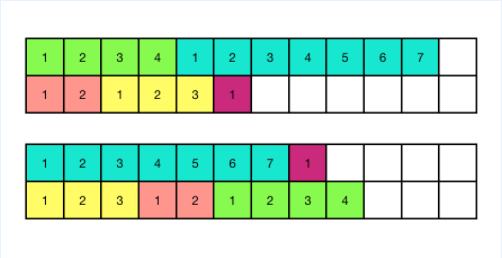
\includegraphics [width =0.4\textwidth]{nucleos.png}
\caption{Número de núcleos y tareas asignadas}
\end{figure}
\end{multicols}

\section{Código}
Con el siguiente código se examinaron como las diferencias en los tiempos de ejecución de los diferentes ordenamientos cambian cuando se varía el número de núcleos asignados al clúster, utilizando como datos de entrada un vector que contiene primos grandes.\\ 
Para conseguir ese vector, se realizó un programa que lee el archivo .txt que se descargó del sitio web\cite{Denisse_L}, el programa convierte el .txt a CSV permitiendo que elijas el rango de números que deseas procesar. A demás el programa te calcula los números no primos, los números pares, y te genera otras 3 columnas que es una combinación de primos- no primos (50\% c/u), no primos- primos (50\% c/u) y aleatorio.\\
\newpage
\definecolor{codegreen}{rgb}{0,0.6,0}
\definecolor{codegray}{rgb}{0.5,0.5,0.5}
\definecolor{codepurple}{rgb}{0.58,0,0.82}
\definecolor{backcolour}{rgb}{0.95,0.95,0.92}

\lstdefinestyle{mystyle}{
    backgroundcolor=\color{backcolour},   
    commentstyle=\color{codegreen},
    keywordstyle=\color{magenta},
    numberstyle=\tiny\color{codegray},
    stringstyle=\color{codepurple},
    basicstyle=\ttfamily\footnotesize,
    breakatwhitespace=false,         
    breaklines=true,                 
    captionpos=b,                    
    keepspaces=true,                 
    numbers=left,                    
    numbersep=5pt,                  
    showspaces=false,                
    showstringspaces=false,
    showtabs=false,                  
    tabsize=2
}
\lstset{style=mystyle}
\begin{lstlisting}[language=Python, caption= Código para convertir de txt a CSV]

#Abrir el archivo txt y convertirlo a un unico vector
with open('primes3.txt', 'r') as in_file:
        for line in in_file:
            if line != '\n':
                txt = re.split(r'\D',line)
                lines.append(txt)
print(len(lines[1]))
#Del vector lines, se eliminan las celdas vacias dejando solo los numeros primos
for x in range(1, len(lines)):
    for y in range(len(lines[x])):
        if lines[x][y] != '':
            primo.append(int(lines[x][y]))

\end{lstlisting}

Estas 6 columnas que se crearon en la matriz se utilizaron para dar tareas de mayor a menor dificultad, esto con la finalidad de medir el tiempo de ejecución en los diferentes núcleos. El código base utilizado en esta tarea se obtuvo del repositorio de la Dra. Schaeffer \cite{Elisa_Schaeffer}

La dificultad que se asignó a cada variante quedo de la siguiente manera (los niveles de dificultad se leen del 1 al 6 tomando a 1 como el más difícil y el 6 el menos difícil):

\begin{table}[h!]
\centering
 \begin{tabular}{||c c ||} 
 \hline
 Nivel de Dificultad & Variantes  \\ [0.5ex] 
 \hline\hline
 1 & Primos \\
 \hline
 2 & Primos- No primos\\ 
 \hline
 3 & No primos - Primos  \\
 \hline
 4 & Aleatorio \\
 \hline
 5 & No primos \\
 \hline
 6 & Pares \\ [1ex] 
 \hline
\end{tabular}
\caption{Relación de dificultad}
\label{table:1}
\end{table}

\begin{lstlisting}[language=Python, caption= Código para obtener los números primos y extraer los datos del CSV.]

def primo(n):
    if n < 4:
        return True
    if n % 2 == 0:
        return False
    for i in range(3, int(ceil(sqrt(n))), 2):
        if n % i == 0:
            return False
    return True
from scipy.stats import describe # instalar con pip3
import multiprocessing
cores = multiprocessing.cpu_count()
from time import time
if __name__ == "__main__":
    df = pd.read_csv('C:/path')
    primos = df['Primos']
    nprimos = df['No_Primos']
    pares = df['Pares']
    p_np = df['Primos_NoPrimos']
    np_p = df['NoPrimos_Primos']
    aleatorio = df['Aleatorio']
    empezar = df['Pares'][:100]

\end{lstlisting}

\section{Resultados}

En las figuras dos, tres y cuatro se muestran las gráficas caja-bigote del tiempo vs variantes procesando con un núcleo, dos, tres, hasta 6 núcleos, esto con la finalidad de observar la variación en el tiempo total con diferentes dificultades como se mencionó anteriormente, se realizaron 10 repeticiones con un vector de 1000 números.
A demás se muestran las tablas con la estadística medida en tiempo (segundos) para cada variante.


\begin{figure}[H]
\centering
\begin{subfigure}[b]{0.45\linewidth}
\includegraphics[width=\linewidth]{Gráfica_tiempo_1.png}
\caption{Tiempo vs variante con un núcleo}
\end{subfigure}
\begin{subfigure}[b]{0.45\linewidth}
\includegraphics[width=\linewidth]{Gráfica_tiempo_2.png}
\caption{Tiempo vs variante con dos núcleos}
\end{subfigure}
\caption{Gráfica de tiempo vs variante núcleo 1 y 2}
\label{fig:westminster}
\end{figure}

\begin{figure}[H]
\centering
\begin{subfigure}[b]{0.45\linewidth}
\includegraphics[width=\linewidth]{Gráfica_tiempo_3.png}
\caption{Tiempo vs variante con tres núcleos}
\end{subfigure}
\begin{subfigure}[b]{0.45\linewidth}
\includegraphics[width=\linewidth]{Gráfica_tiempo_4.png}
\caption{Tiempo vs variante con cuatro núcleos}
\end{subfigure}
\caption{Gráfica de tiempo vs variante núcleo 3 y 4}
\label{fig:westminster}
\end{figure}

\begin{figure}[H]
\centering
\begin{subfigure}[b]{0.45\linewidth}
\includegraphics[width=\linewidth]{Gráfica_tiempo_5.png}
\caption{Tiempo vs variante con cinco núcleos}
\end{subfigure}
\begin{subfigure}[b]{0.45\linewidth}
\includegraphics[width=\linewidth]{Gráfica_tiempo_6.png}
\caption{Tiempo vs variante con seis núcleos}
\end{subfigure}
\caption{Gráfica de tiempo vs variante núcleo 5 y 6}
\label{fig:westminster}
\end{figure}

\begin{table}[H]
\centering
\begin{tabular}{|l | r | r | r | r | r | r|}
\hline
\multicolumn{7}{|c|}{Un núcleo}\\
\hline
Variante&Iteración&Min-Max&Mediana&Varianza&Asimetría&Curtosis\\
\hline
 Primos               & 10 & 1.51, 1.76   & 1.56 & 0.00 & 2.06& 2.98\\
 Primos - No primos   & 10 & 0.89, 1.07 & 0.93 & 0.00 & 2.35& 4.09\\
 No primos - primos   & 10 & 0.89, 1.11  & 0.95 & 0.00 & 1.48& 0.45\\
 Aleatorio            & 10 & 0.90, 0.98  & 0.93 & 0.00& 0.84& -0.30\\
 No primos            & 10 & 0.30, 0.43  & 0.32 & 0.00 & 2.61& 4.95\\
 Pares                & 10 & 0.0, 0.00  & 0.00 & 1.10 & 0.86& -0.86\\
\hline
\end{tabular}
\caption{Tabla de estadística con un núcleo}
\label{table:1}
\end{table}

\begin{table}[H]
\begin{center}
\begin{tabular}{|l | r | r | r | r | r | r|}
\hline
\multicolumn{7}{|c|}{Dos núcleos}\\
\hline
Variante&Iteración&Min-Max&Mediana&Varianza&Asimetría&Curtosis\\
\hline
 Primos               & 10 & 0.80, 1.10  & 0.91 & 0.01 & 0.40& -1.45\\
 Primos - No primos   & 10 & 0.49, 0.64  & 0.55 & 0.00 & 0.42& -1.60\\
 No primos - primos   & 10 & 0.48, 0.61  & 0.55 & 0.00 & 0.20& -1.74\\
 Aleatorio            & 10 & 0.47, 0.64  & 0.55 & 0.00 & 0.01& -1.66\\
 No primos            & 10 & 0.16, 0.25  & 0.19 & 0.00 & 0.88& -0.11\\
 Pares                & 10 & 0.0, 0.00  & 0.00 & 1.18 & 1.23& -0.06\\
\hline
\end{tabular}
\caption{Tabla de estadística con dos núcleos}
\label{table:1}
\end{center}
\end{table}

\begin{table}[H]
\begin{center}
\begin{tabular}{|l | r | r | r | r | r | r|}
\hline
\multicolumn{7}{|c|}{Tres núcleos}\\
\hline
Variante&Iteración&Min-Max&Mediana&Varianza&Asimetría&Curtosis\\
\hline
 Primos               & 10 & 0.77, 0.97  & 0.83 & 0.00 & 1.47  & 1.12\\
 Primos - No primos   & 10 & 0.47, 0.56 & 0.50   & 0.00 &0.66& -0.16\\
 No primos - primos   & 10 & 0.44, 0.57  &0.48 & 0.00 & 1.08& 0.40\\
 Aleatorio            & 10 & 0.47, 0.56  & 0.50 & 0.00 &0.98& 0.05\\
 No primos            & 10 & 0.15, 0.20  & 0.17 & 0.00 & 0.97&0.44\\
 Pares                & 10 & 0.0, 0.01  & 0.00 & 1.13 & 0.39& -1.18\\
\hline
\end{tabular}
\caption{Tabla de estadística con tres núcleos}
\label{table:1}
\end{center}
\end{table}

\begin{table}[H]
\begin{center}
\begin{tabular}{|l | r | r | r | r | r | r|}
\hline
\multicolumn{7}{|c|}{Cuatro núcleos}\\
\hline
Variante&Iteración&Min-Max&Mediana&Varianza&Asimetría&Curtosis\\
\hline
 Primos               & 10 & 0.69, 0.83  & 0.76 & 0.00 & 0.24  & -0.82\\
 Primos - No primos   & 10 & 0.42, 0.51  & 0.46 & 0.00 & 0.36  & -1.29\\
 No primos - primos   & 10 & 0.42, 0.49  &0.45 & 0.00 & 0.35   & -1.42\\
 Aleatorio            & 10 & 0.42, 0.52  & 0.46 & 0.00 &0.36   & -0.78\\
 No primos            & 10 & 0.14, 0.18  & 0.16 & 0.00 & 0.21  &0.71\\
 Pares                & 10 & 0.0, 0.00  & 0.00 & 8.98 & 0.15   & -1.35\\
\hline
\end{tabular}
\caption{Tabla de estadística con cuatro núcleos}
\label{table:1}
\end{center}
\end{table}

\begin{table}[H]
\begin{center}
\begin{tabular}{|l | r | r | r | r | r | r|}
\hline
\multicolumn{7}{|c|}{Cinco núcleos}\\
\hline
Variante&Iteración&Min-Max&Mediana&Varianza&Asimetría&Curtosis\\
\hline
 Primos               & 10 & 0.74, 0.86  & 0.77 & 0.00 & 1.86  & 2.52\\
 Primos - No primos   & 10 & 0.42, 0.47  & 0.45 & 0.00 & 0.09  & -0.65\\
 No primos - primos   & 10 & 0.42, 0.49  &0.46 & 0.00 & 0.01   & -0.90\\
 Aleatorio            & 10 & 0.42, 0.50  & 0.45 & 0.00 &1.11   & 1.21\\
 No primos            & 10 & 0.14, 0.18  & 0.15 & 0.00 & 0.26  &-1.19\\
 Pares                & 10 & 0.0, 0.00  & 0.00 & 6.49 & -1.21   & 0.35\\
\hline
\end{tabular}
\caption{Tabla de estadística con cinco núcleos}
\label{table:1}
\end{center}
\end{table}

\begin{table}[H]
\begin{center}
\begin{tabular}{|l | r | r | r | r | r | r|}
\hline
\multicolumn{7}{|c|}{Seis núcleos}\\
\hline
Variante&Iteración&Min-Max&Mediana&Varianza&Asimetría&Curtosis\\
\hline
 Primos               & 10 & 0.68, 0.75  & 0.70 & 0.00 & 0.94   & 0.56\\
 Primos - No primos   & 10 & 0.39, 0.43  & 0.41 & 0.00 & -0.25  & 0.03\\
 No primos - primos   & 10 & 0.42, 0.46  &0.44 & 0.00  & 0.67   & -1.01\\
 Aleatorio            & 10 & 0.39, 0.50  & 0.42 & 0.00 & 1.31   & 1.36\\
 No primos            & 10 & 0.14, 0.15  & 0.14 & 4.51 & 1.12   &-0.32\\
 Pares                & 10 & 0.0, 0.00  & 0.00 & 8.99  & -1.59  & 0.67\\
\hline
\end{tabular}
\caption{Tabla de estadística con seis núcleos}
\label{table:1}
\end{center}
\end{table}

\section{Reto 1}
Para este reto se modifica el código anterior para que encuentre todos los divisores del número (es decir, todos los enteros mayores a uno y menores al número mismo que lo dividen exactamente) y examinar si las conclusiones cambian.

En este código también se usó un vector de 1000 números, solo que en esta ocasión fueron 30 repeticiones. El código completo en Python se encuentra en el GitHub \cite{Denisse_Leyva}.
En las figuras cinco, seis y siete se muestras las gráficas caja-bigote del tiempo vs variantes para la obtención de los divisores, así como las tablas estadísticas para uno, dos, tres, cuatro, cinco y seis núcleos.

\begin{figure}[H]
\centering
\begin{subfigure}[b]{0.45\linewidth}
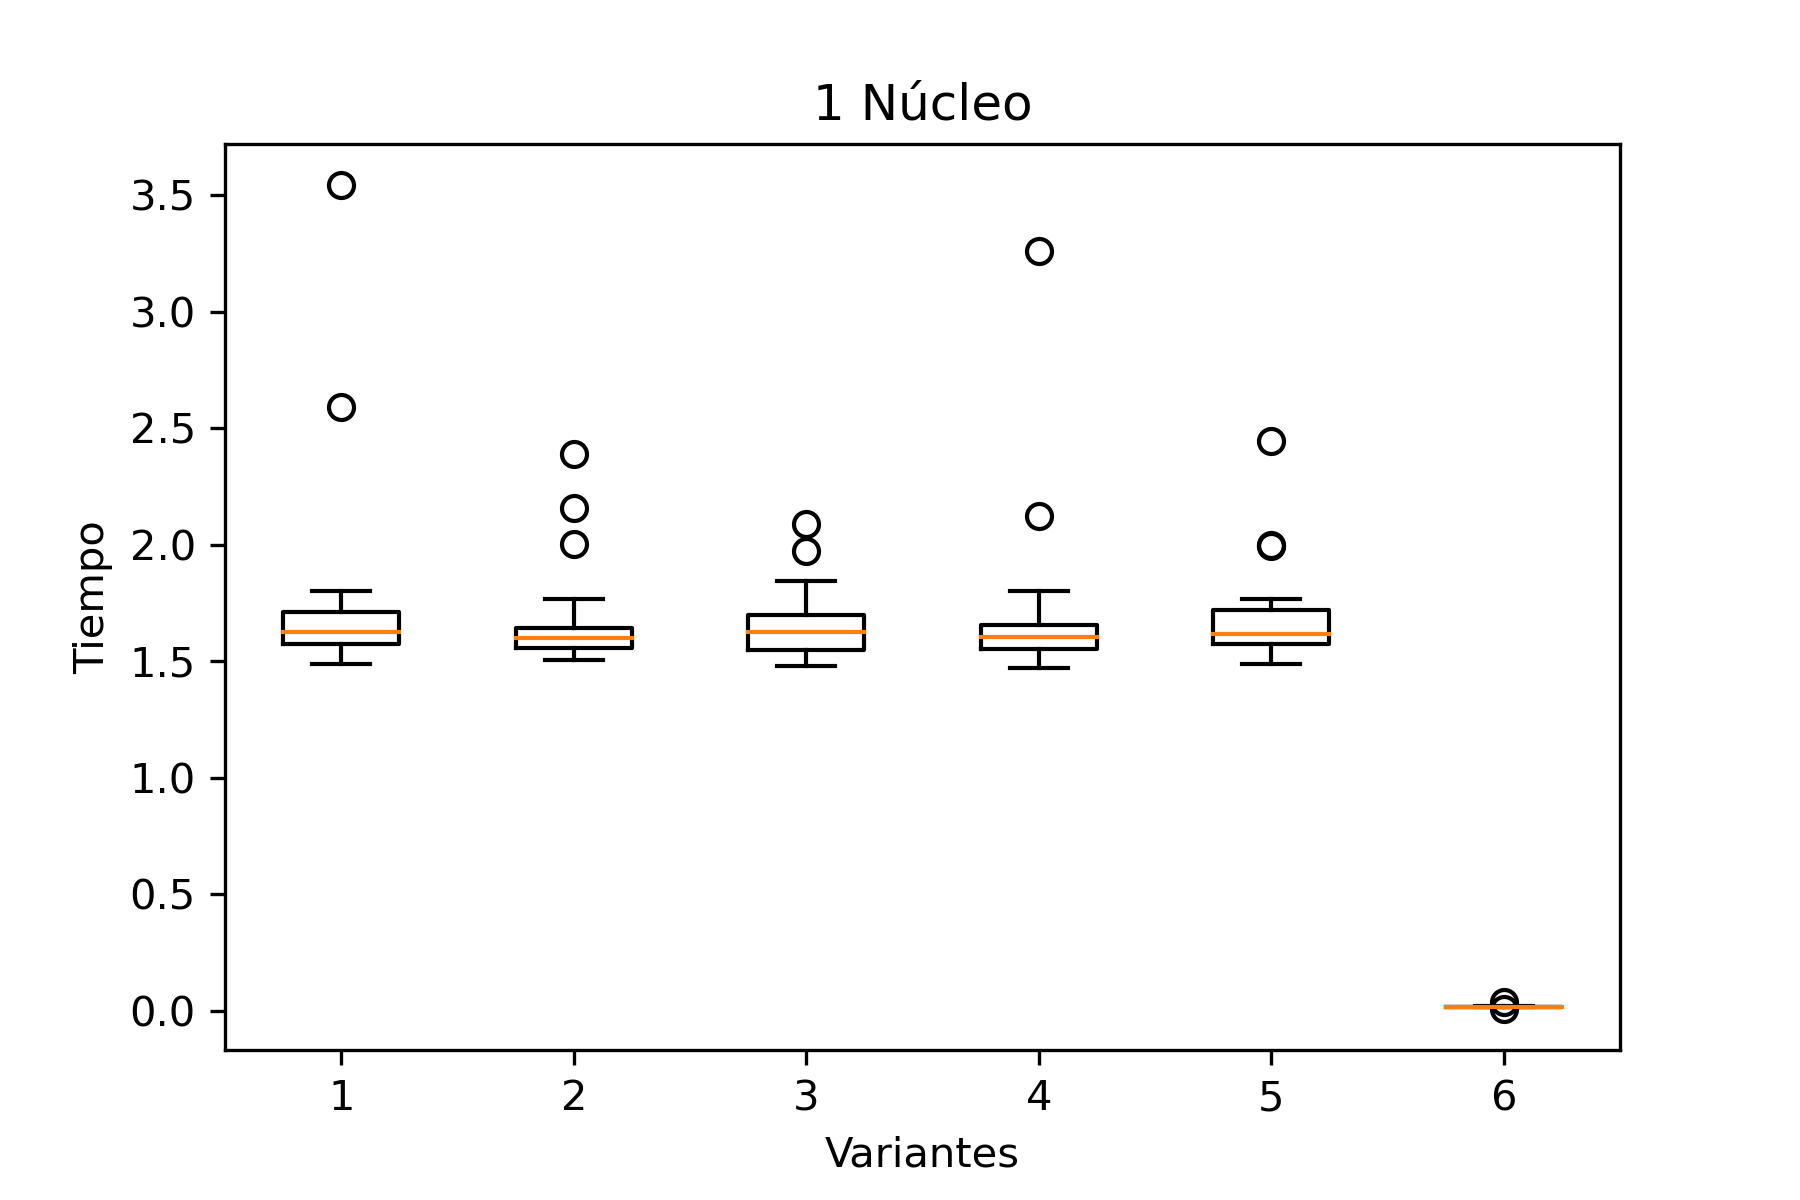
\includegraphics[width=\linewidth]{Gráfica_1.png}
\caption{Tiempo vs variante con un núcleo}
\end{subfigure}
\begin{subfigure}[b]{0.45\linewidth}
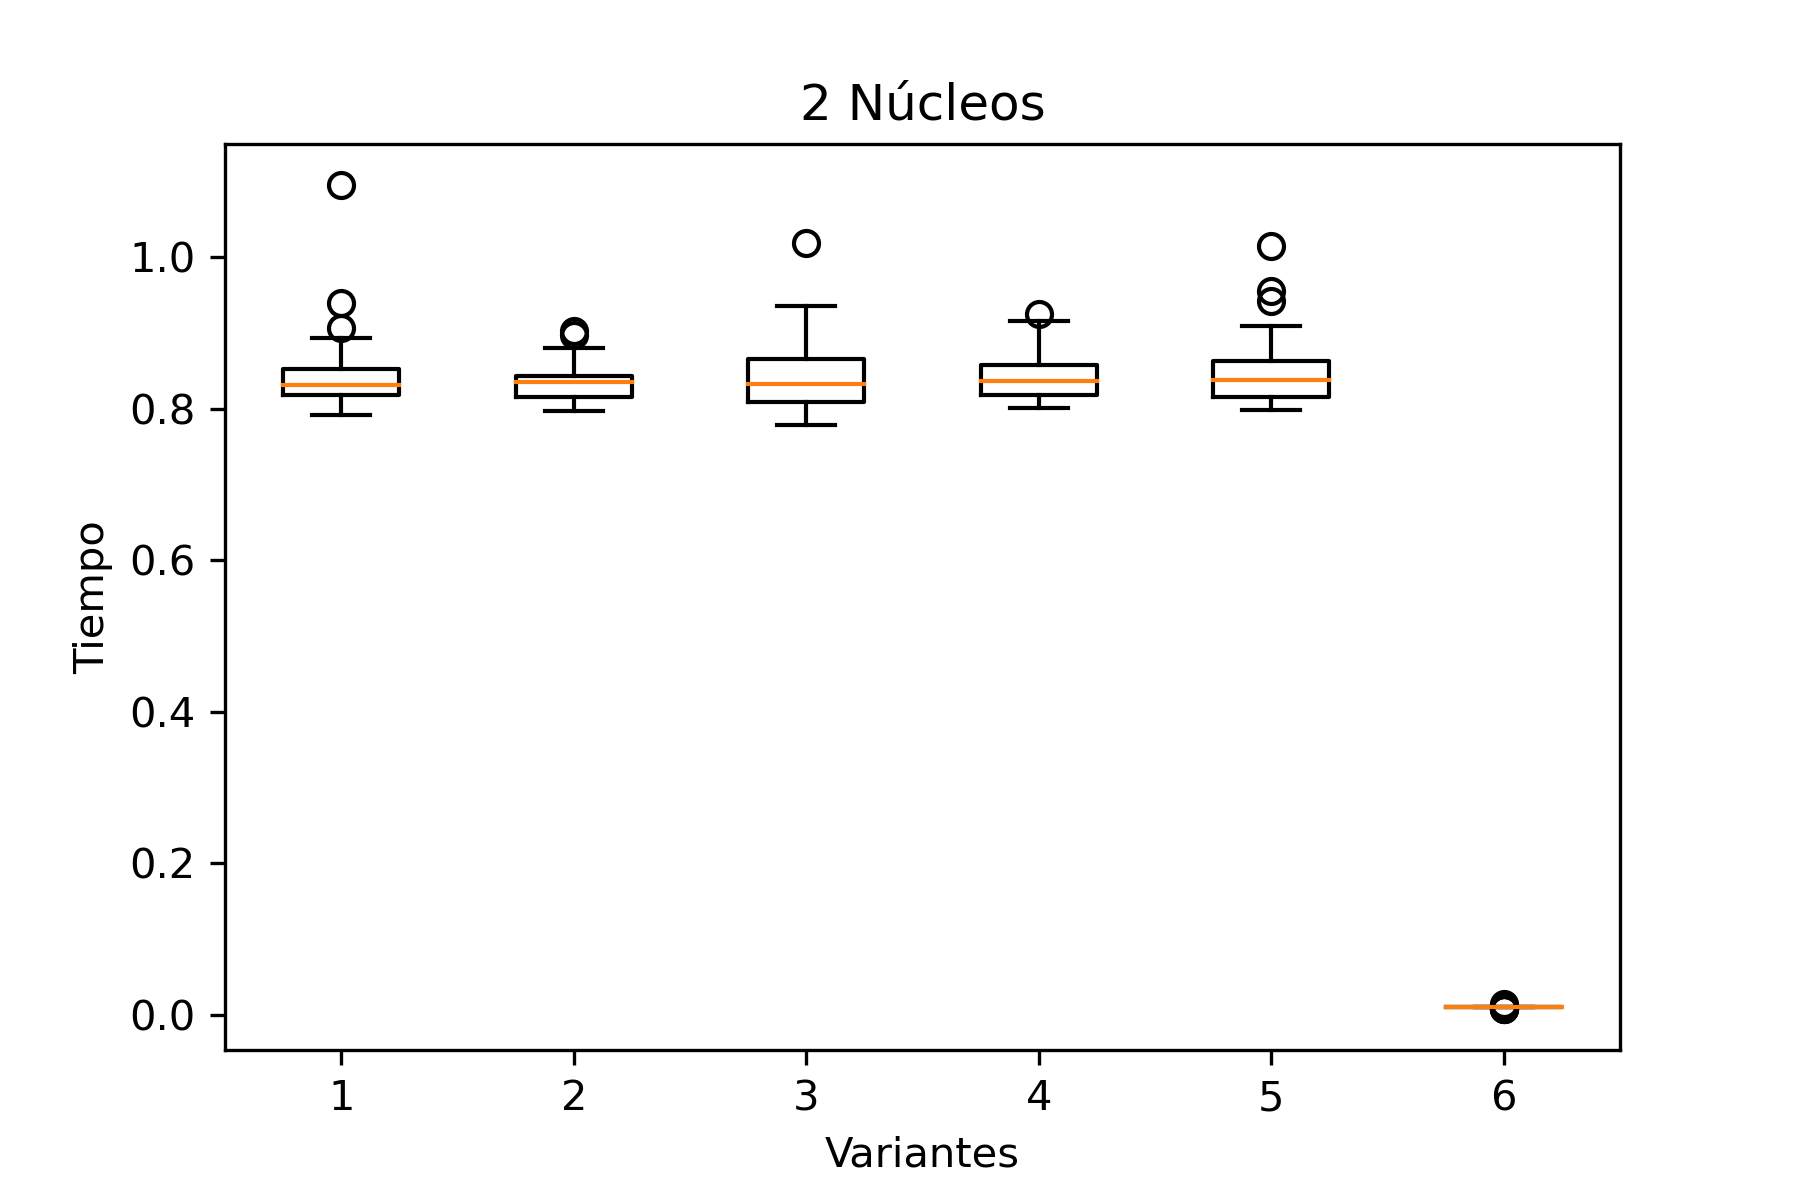
\includegraphics[width=\linewidth]{Gráfica_2.png}
\caption{Tiempo vs variante con dos núcleos}
\end{subfigure}
\caption{Gráfica de tiempo vs variante núcleo 1 y 2 para obtención de divisores.}
\label{fig:westminster}
\end{figure}

\begin{figure}[H]
\centering
\begin{subfigure}[b]{0.45\linewidth}
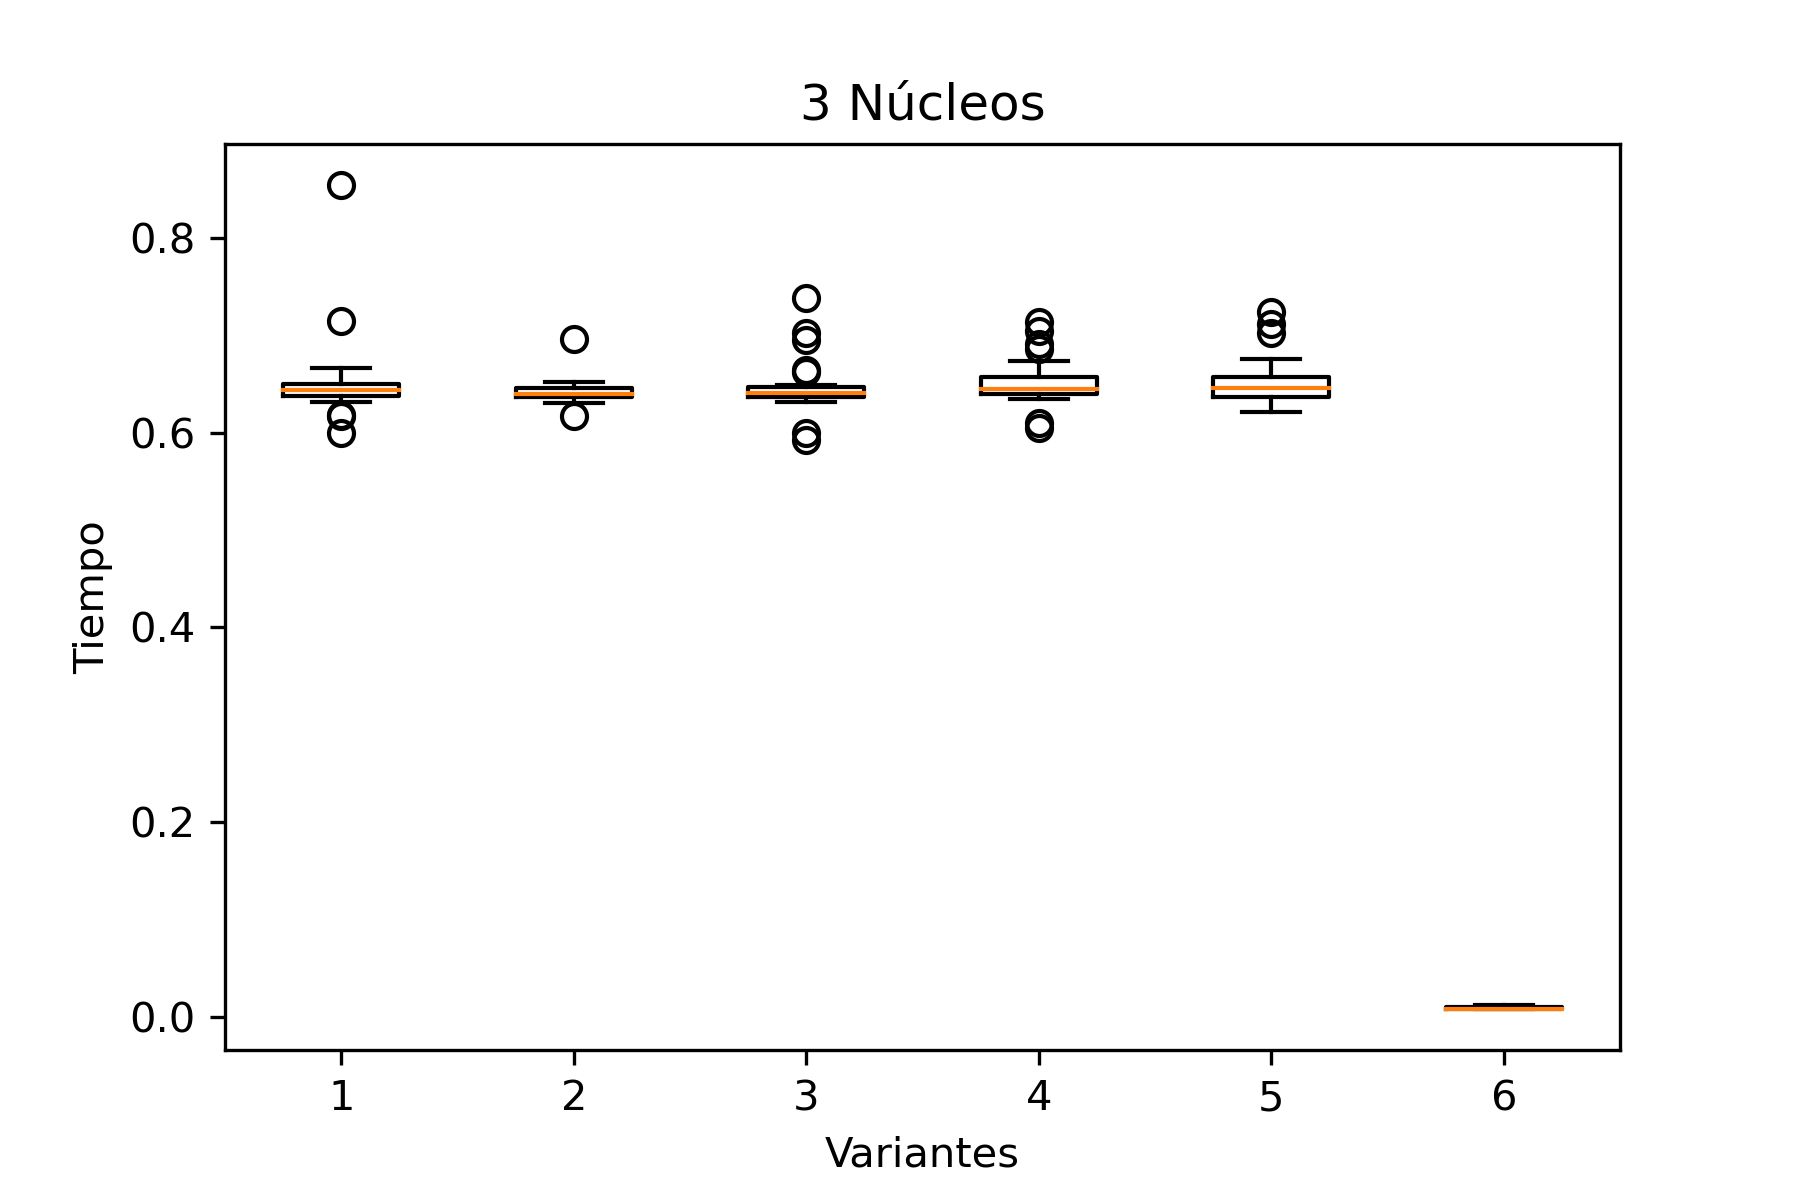
\includegraphics[width=\linewidth]{Gráfica_3.png}
\caption{Tiempo vs variante con tres núcleos}
\end{subfigure}
\begin{subfigure}[b]{0.45\linewidth}
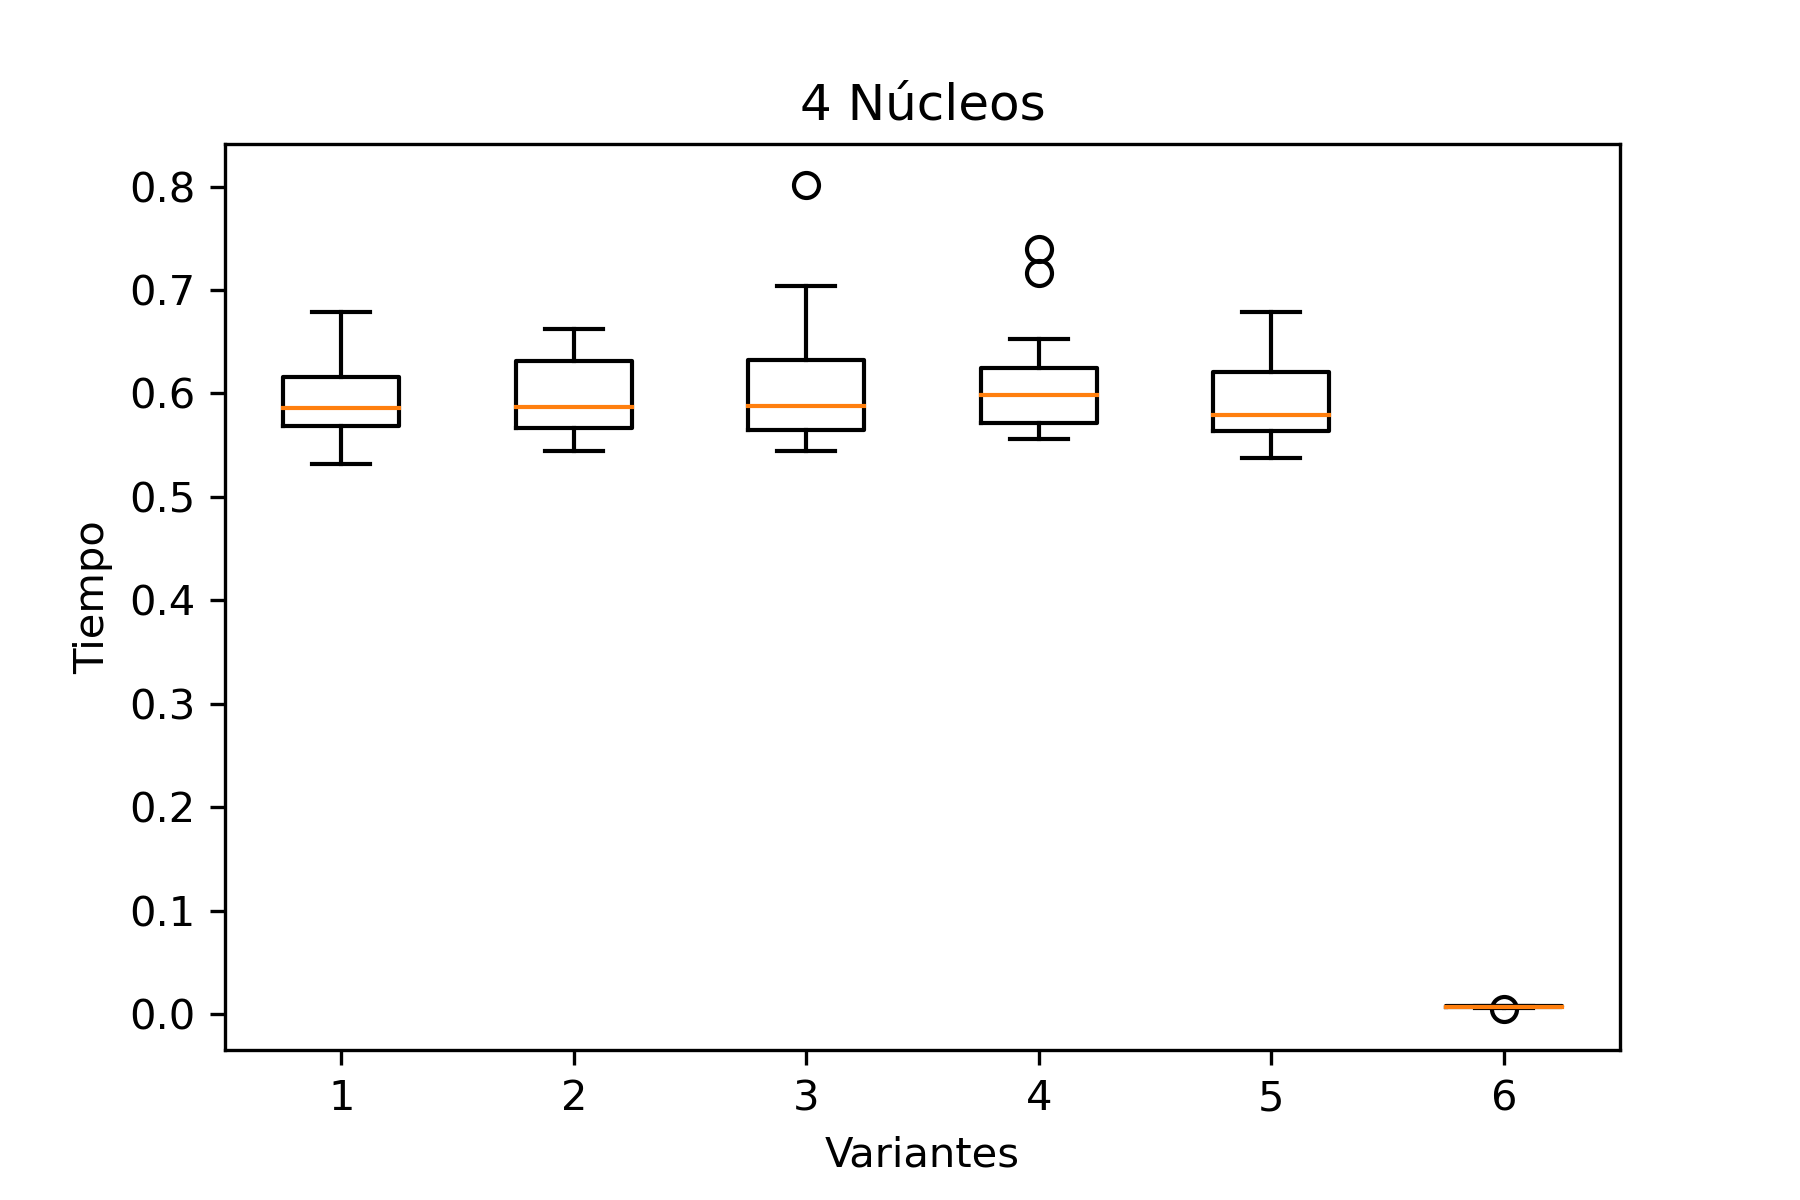
\includegraphics[width=\linewidth]{Gráfica_4.png}
\caption{Tiempo vs variante con cuatro núcleos}
\end{subfigure}
\caption{Gráfica de tiempo vs variante núcleo 3 y 4 para obtención de divisores.}
\label{fig:westminster}
\end{figure}

\begin{figure}[H]
\centering
\begin{subfigure}[b]{0.45\linewidth}
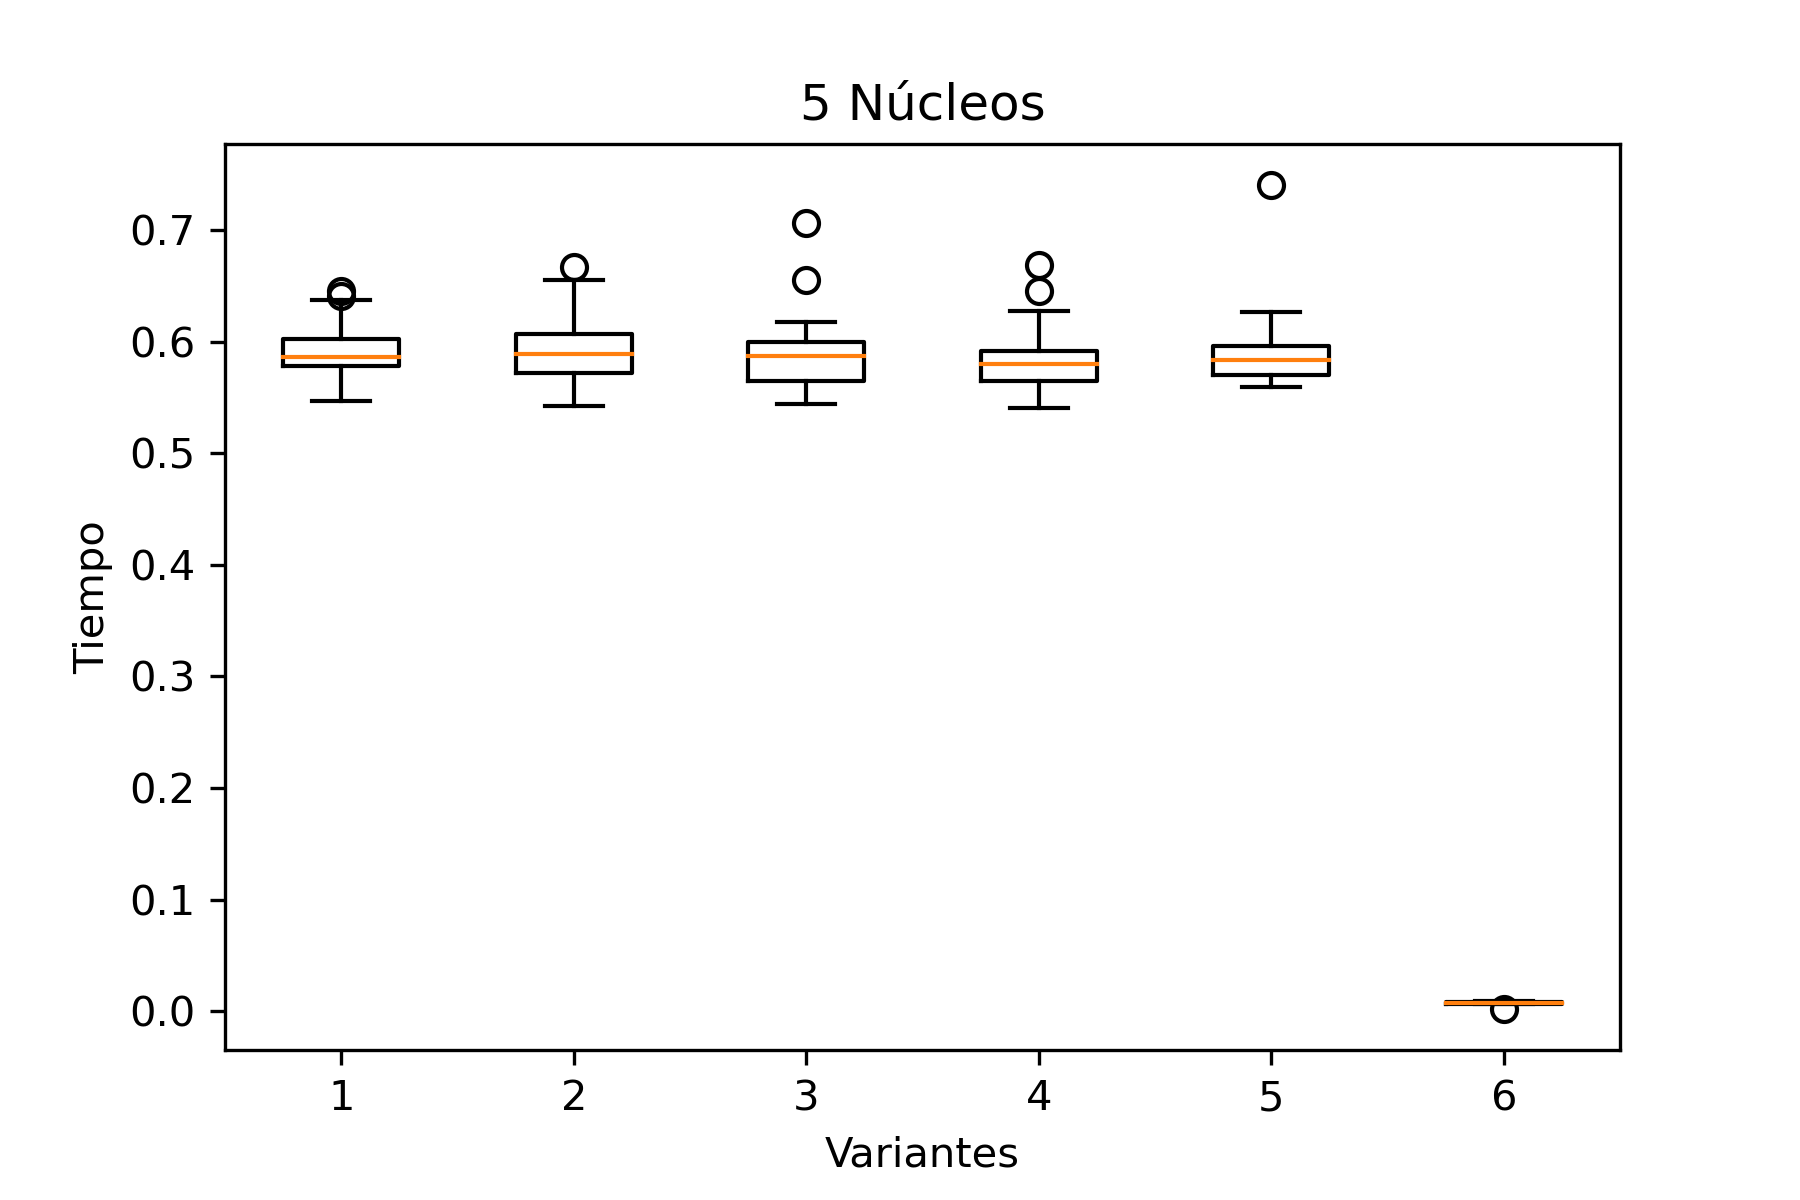
\includegraphics[width=\linewidth]{Gráfica_5.png}
\caption{Tiempo vs variante con cinco núcleos}
\end{subfigure}
\begin{subfigure}[b]{0.45\linewidth}
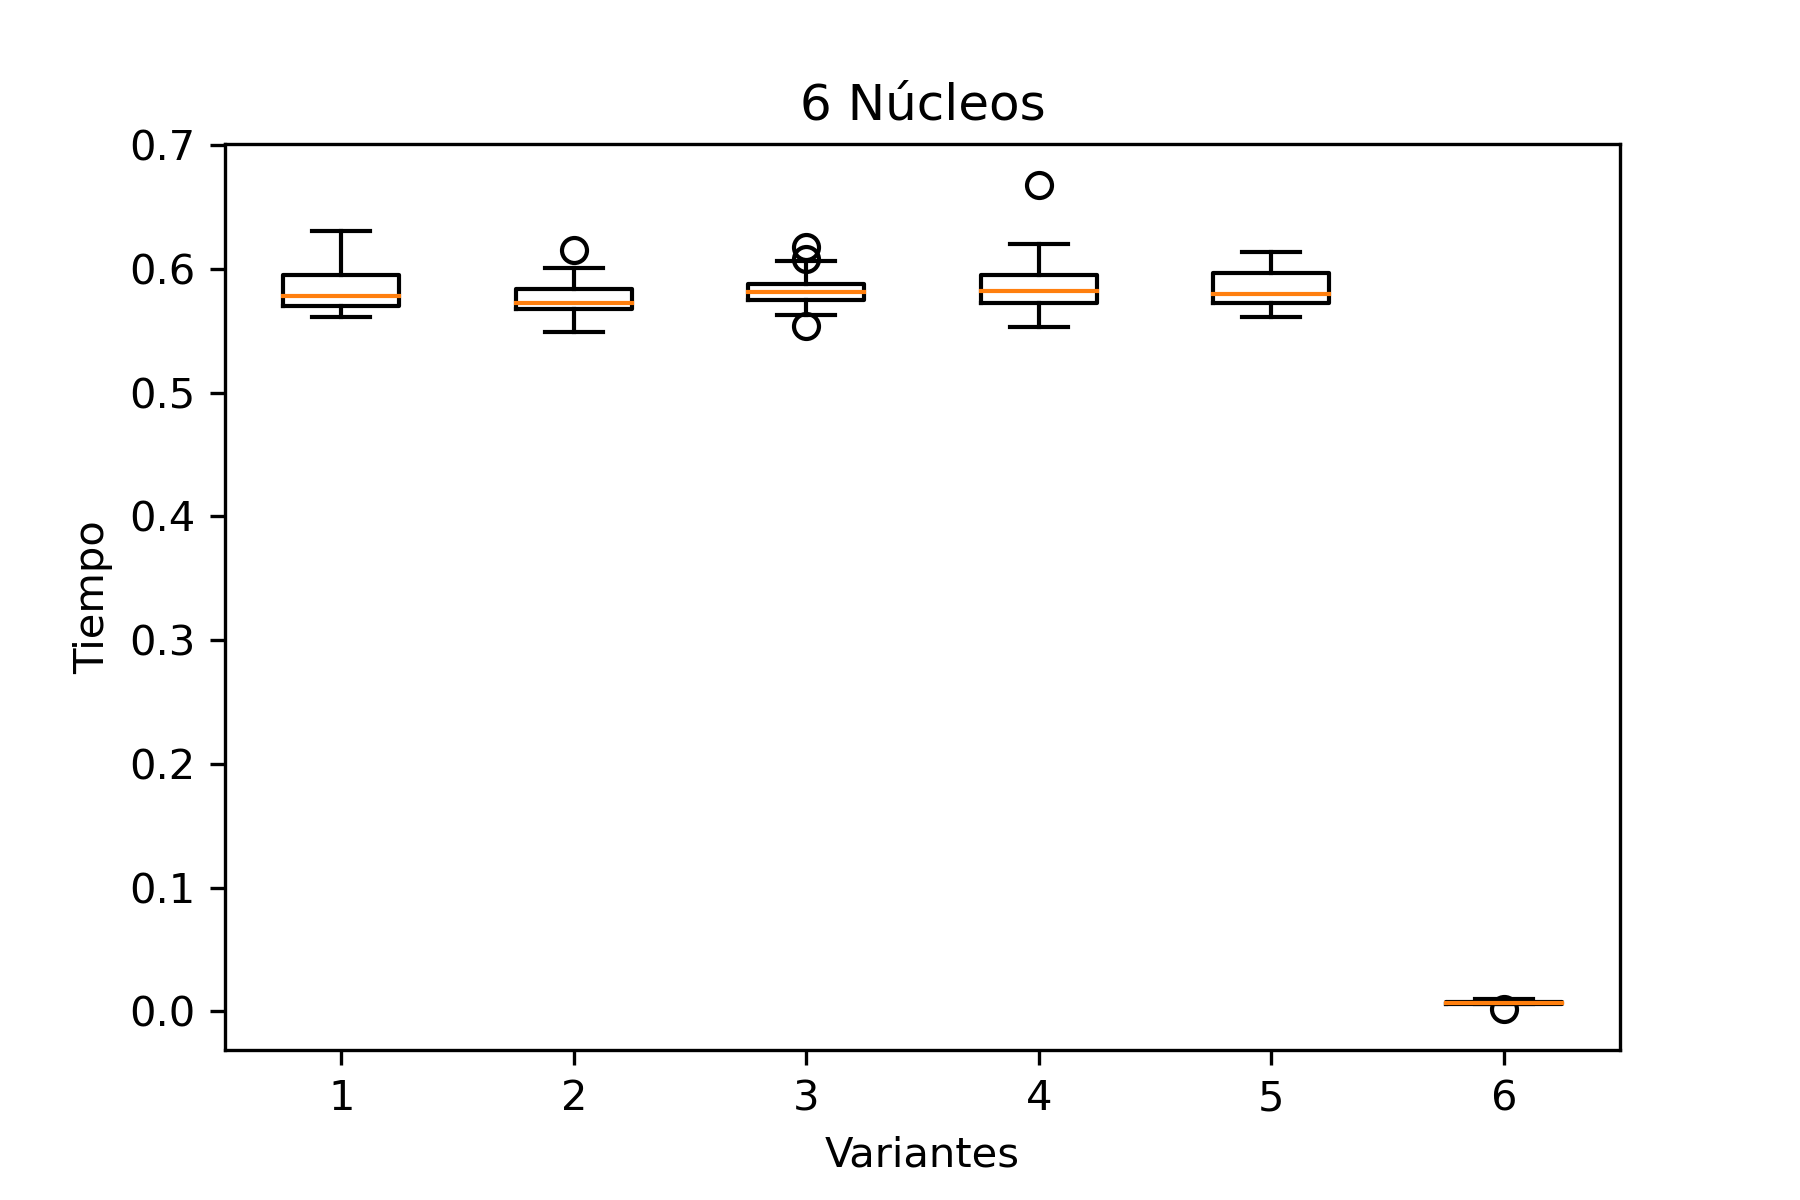
\includegraphics[width=\linewidth]{Gráfica_6.png}
\caption{Tiempo vs variante con seis núcleos}
\end{subfigure}
\caption{Gráfica de tiempo vs variante núcleo 5 y 6 para obtención de divisores.}
\label{fig:westminster}
\end{figure}

\begin{table}[H]
\begin{center}
\begin{tabular}{|l | r | r | r | r | r | r|}
\hline
\multicolumn{7}{|c|}{Un núcleo}\\
\hline
Variante&iteración&Min-Max&Mediana&Varianza&Asimetría&Curtosis\\
\hline
 Primos               & 30 & 1.48, 3.54  & 1.72 & 0.15 & 3.76   & 13.98\\
 Primos - No primos   & 30 & 1.54, 2.38  & 1.65 & 0.03 & 2.62   & 6.32\\
 No primos - primos   & 30 & 1.47, 2.08  & 1.64 & 0.01  & 1.47  & 2.14\\
 Aleatorio            & 30 & 1.46, 3.25  & 1.68 & 0.10 & 4.12   & 17.41\\
 No primos            & 30 & 1.48, 2.44  & 1.67 & 0.03 & 2.56   & 7.38\\
 Pares                & 30 & 0.00, 0.03  & 0.01 & 1.62  & 2.89  & 13.71\\
\hline
\end{tabular}
\caption{Tabla de estadística con un núcleo }
\label{table:1}
\end{center}
\end{table}

\begin{table}[H]
\begin{center}
\begin{tabular}{|l | r | r | r | r | r | r|}
\hline
\multicolumn{7}{|c|}{Dos núcleos}\\
\hline
Variante&iteración&Min-Max&Mediana&Varianza&Asimetría&Curtosis\\
\hline
 Primos               & 30 & 0.79, 1.09  & 0.84 & 0.00 & 3.01   & 10.39\\
 Primos - No primos   & 30 & 0.79, 0.90  & 0.83 & 0.00 & 0.73   & 0.46\\
 No primos - primos   & 30 & 0.77, 1.01  & 0.84 & 0.00  & 1.69  & 3.58\\
 Aleatorio            & 30 & 0.80, 0.92  & 0.84 & 0.00 & 0.88   & 0.09\\
 No primos            & 30 & 0.79, 1.01  & 0.85 & 0.00 & 1.62   & 2.45\\
 Pares                & 30 & 0.00, 0.01  & 0.01 & 1.27  & 1.06  & 3.84\\
\hline
\end{tabular}
\caption{Tabla de estadística con dos núcleos}
\label{table:1}
\end{center}
\end{table}

\begin{table}[H]
\begin{center}
\begin{tabular}{|l | r | r | r | r | r | r|}
\hline
\multicolumn{7}{|c|}{Tres núcleos}\\
\hline
Variante&iteración&Min-Max&Mediana&Varianza&Asimetría&Curtosis\\
\hline
 Primos               & 30 & 0.59, 0.85  & 0.65 & 0.00 & 3.80   & 15.64\\
 Primos - No primos   & 30 & 0.61, 0.69  & 0.64 & 0.00 & 2.54   & 10.11\\
 No primos - primos   & 30 & 0.59, 0.73  & 0.64 & 0.00  & 1.50  & 3.99\\
 Aleatorio            & 30 & 0.60, 0.71  & 0.65 & 0.00 & 0.83   & 0.95\\
 No primos            & 30 & 0.62, 0.72  & 0.65 & 0.00 & 1.67   & 2.31\\
 Pares                & 30 & 0.00, 0.01  & 0.00 & 2.07  & 0.90  & -0.82\\
\hline
\end{tabular}
\caption{Tabla de estadística con tres núcleos}
\label{table:1}
\end{center}
\end{table}

\begin{table}[H]
\begin{center}
\begin{tabular}{|l | r | r | r | r | r | r|}
\hline
\multicolumn{7}{|c|}{Cuatro núcleos}\\
\hline
Variante&iteración&Min-Max&Mediana&Varianza&Asimetría&Curtosis\\
\hline
 Primos               & 30 & 0.53, 0.67  & 0.59 & 0.00 & 0.56   & 0.23\\
 Primos - No primos   & 30 & 0.54, 0.66  & 0.59 & 0.00 & 0.39   & -1.14\\
 No primos - primos   & 30 & 0.54, 0.80  & 0.60 & 0.00  & 1.82  & 4.02\\
 Aleatorio            & 30 & 0.55, 0.73  & 0.60 & 0.00 & 1.35   & 1.71\\
 No primos            & 30 & 0.53, 0.67  & 0.59 & 0.00 & 0.55   & 0.78\\
 Pares                & 30 & 0.00, 0.00  & 0.00 & 6.39 & 0.46  & -0.32\\
\hline
\end{tabular}
\caption{Tabla de estadística con cuatro núcleos}
\label{table:1}
\end{center}
\end{table}

\begin{table}[H]
\begin{center}
\begin{tabular}{|l | r | r | r | r | r | r|}
\hline
\multicolumn{7}{|c|}{Cinco núcleos}\\
\hline
Variante&iteración&Min-Max&Mediana&Varianza&Asimetría&Curtosis\\
\hline
 Primos               & 30 & 0.54, 0.64  & 0.59 & 0.00 & 0.58   & 0.37\\
 Primos - No primos   & 30 & 0.54, 0.66  & 0.59 & 0.00 & 0.57   & 0.46\\
 No primos - primos   & 30 & 0.54, 0.70  & 0.58 & 0.00  & 1.63  & 3.88\\
 Aleatorio            & 30 & 0.54, 0.66  & 0.58 & 0.00 & 1.03   & 1.03\\
 No primos            & 30 & 0.55, 0.74  & 0.58 & 0.00 & 3.19   & 12.21\\
 Pares                & 30 & 0.00, 0.00  & 0.00 & 1.67 & -1.60  & 4.60\\
\hline
\end{tabular}
\caption{Tabla de estadística con cinco núcleos}
\label{table:1}
\end{center}
\end{table}

\begin{table}[H]
\begin{center}
\begin{tabular}{|l | r | r | r | r | r | r|}
\hline
\multicolumn{7}{|c|}{Seis núcleos}\\
\hline
Variante&iteración&Min-Max&Mediana&Varianza&Asimetría&Curtosis\\
\hline
 Primos               & 30 & 0.56, 0.63  & 0.58 & 0.00 & 0.93   & -0.25\\
 Primos - No primos   & 30 & 0.54, 0.61  & 0.57 & 0.00 & 0.52   & 0.23\\
 No primos - primos   & 30 & 0.55, 0.61  & 0.58 & 0.00  &0.52  &  0.39\\
 Aleatorio            & 30 & 0.55, 0.66  & 0.58 & 0.00 & 1.59   & 3.91\\
 No primos            & 30 & 0.56, 0.61  & 0.58 & 0.00 & 0.37   & -0.98\\
 Pares                & 30 & 0.00, 0.01  & 0.00 & 1.98 & -0.76  & 4.18\\
\hline
\end{tabular}
\caption{Tabla de estadística con seis núcleos}
\label{table:1}
\end{center}
\end{table}

\section{Reto 2}
Para este reto se modificó el primer reto a que encuentre solamente los factores y sus multiplicidades, es decir, que encuentre para n aquellos numeros primos mayores a 1 y menores o iguales a n y sus potencias para el producto de los factores con esas potencias de n.

Para obtener las gráficas de la 8 a la 10 se utilizó un vector con 1000 números y 40 repeticiones para la obtención de los divisores primos y las potencias de estos mismos. A demás de las tablas estadísticas con uno, dos, tres, cuatro, cinco y seis núcleos. El código completo esta en Github \cite{Denisse_Leyva}.

\begin{figure}[H]
\centering
\begin{subfigure}[b]{0.45\linewidth}
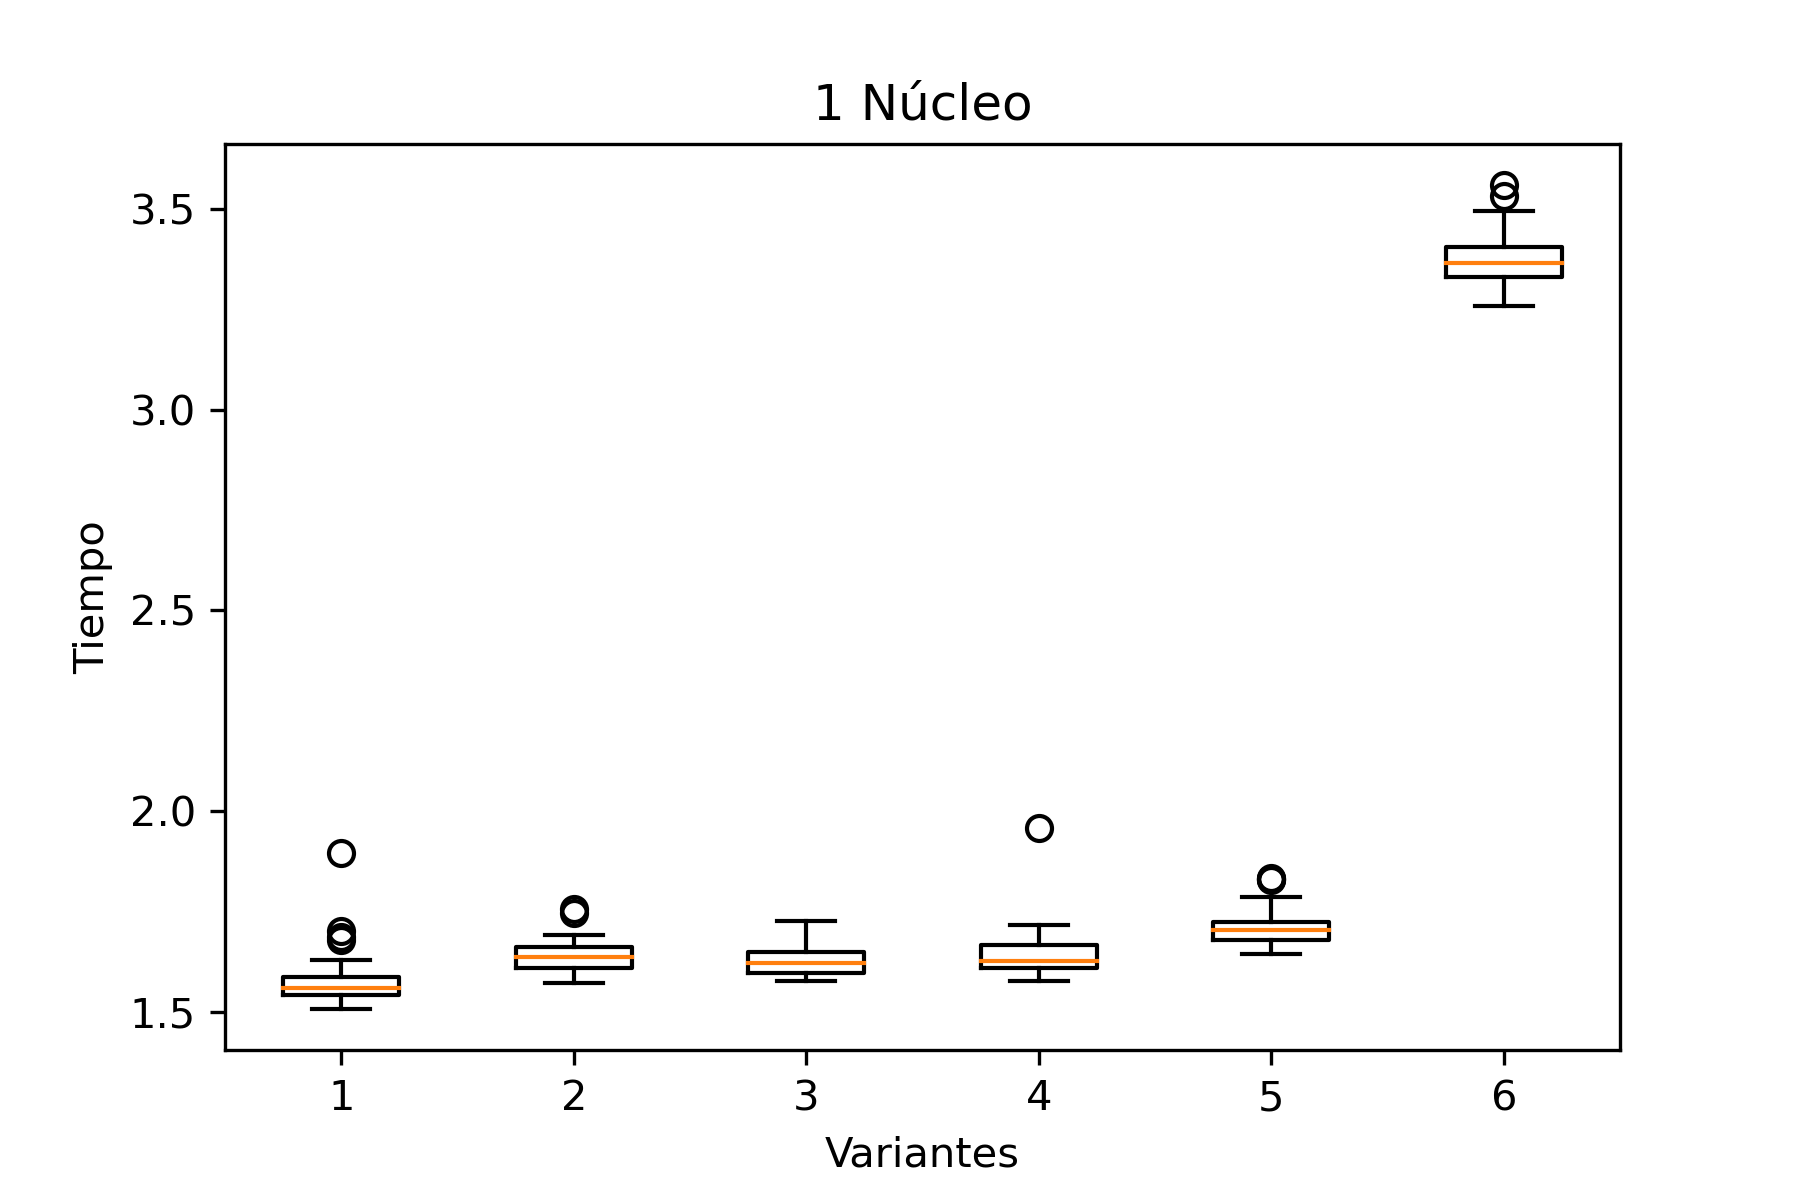
\includegraphics[width=\linewidth]{G_tiempo_1.png}
\caption{Tiempo vs variante con un núcleo}
\end{subfigure}
\begin{subfigure}[b]{0.45\linewidth}
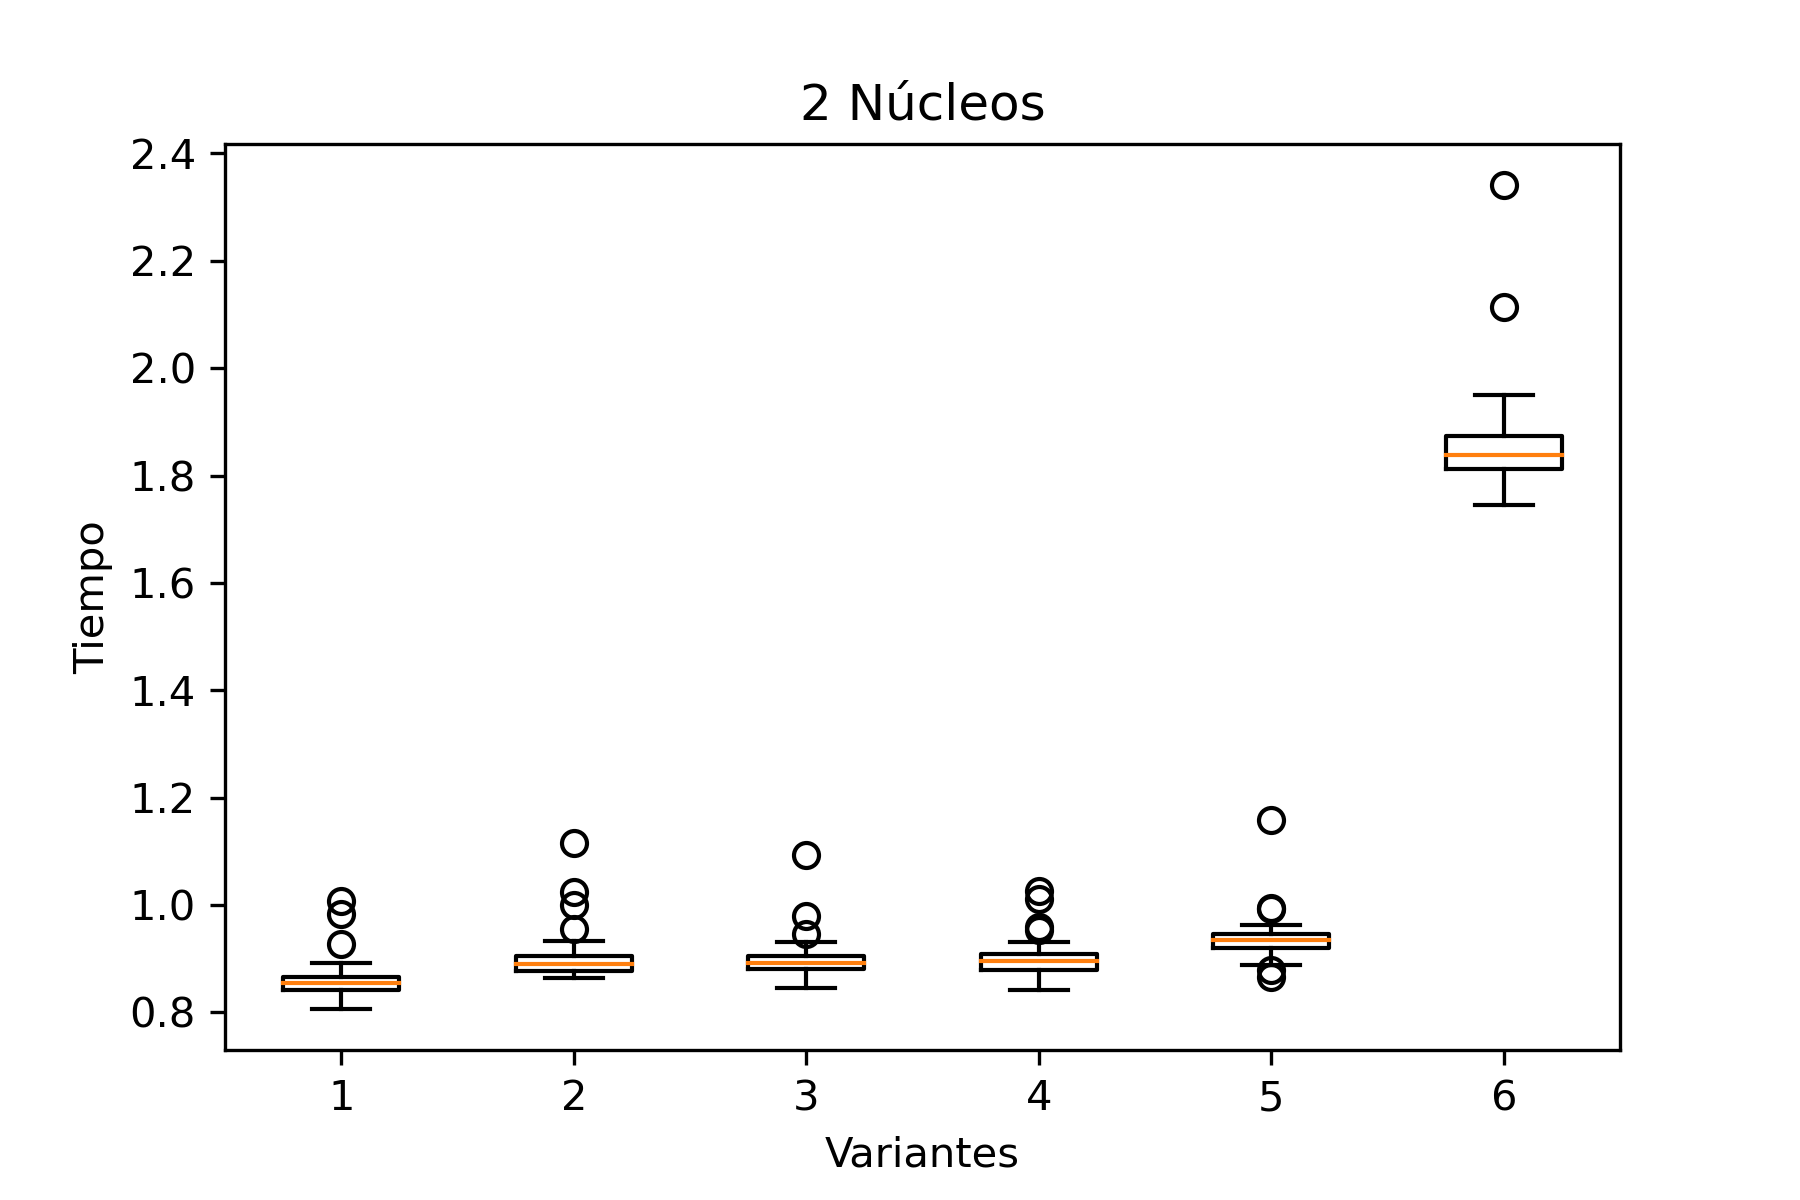
\includegraphics[width=\linewidth]{G_tiempo_2.png}
\caption{Tiempo vs variante con dos núcleos}
\end{subfigure}
\caption{Gráfica de tiempo vs variante núcleo 1 y 2 para obtención de números primos y sus potencias.}
\label{fig:westminster}
\end{figure}

\begin{figure}[H]
\centering
\begin{subfigure}[b]{0.45\linewidth}
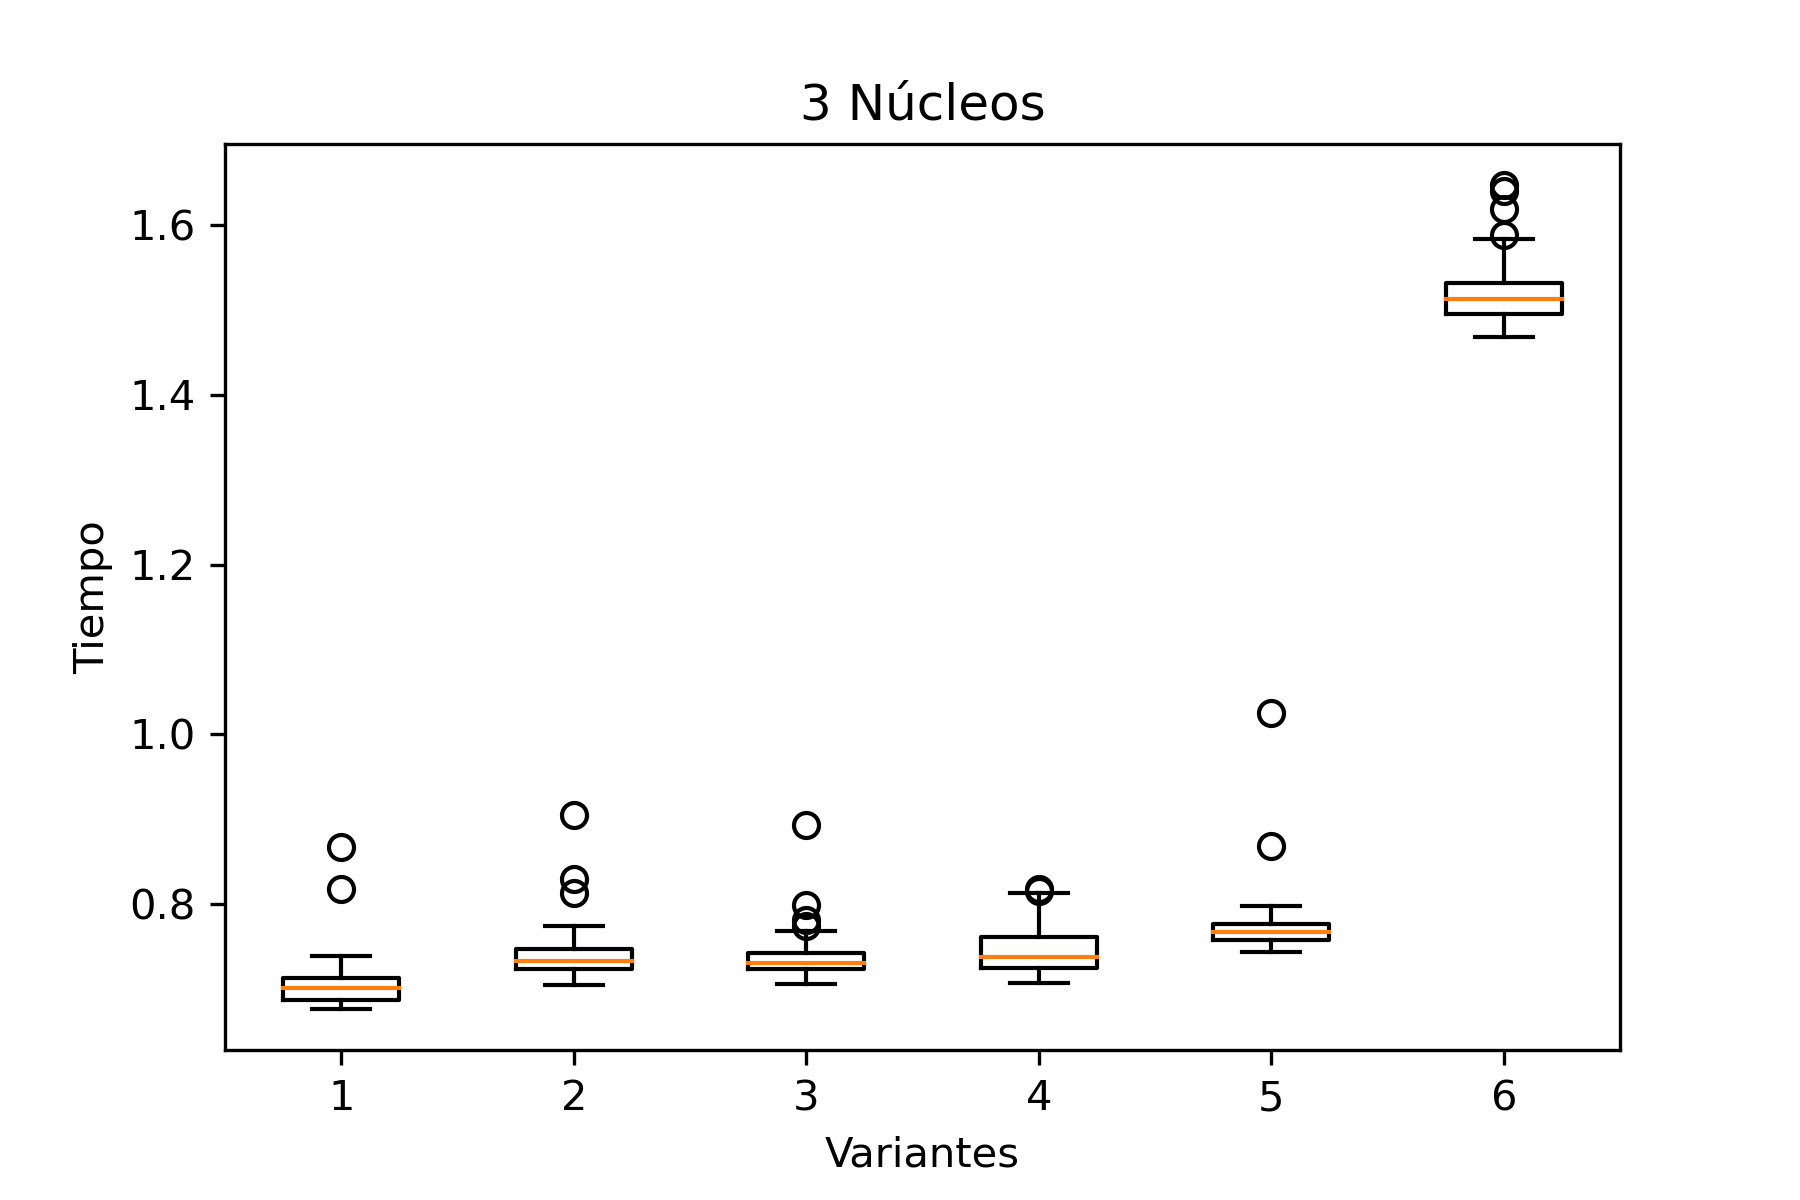
\includegraphics[width=\linewidth]{G_tiempo_3.png}
\caption{Tiempo vs variante con tres núcleos}
\end{subfigure}
\begin{subfigure}[b]{0.45\linewidth}
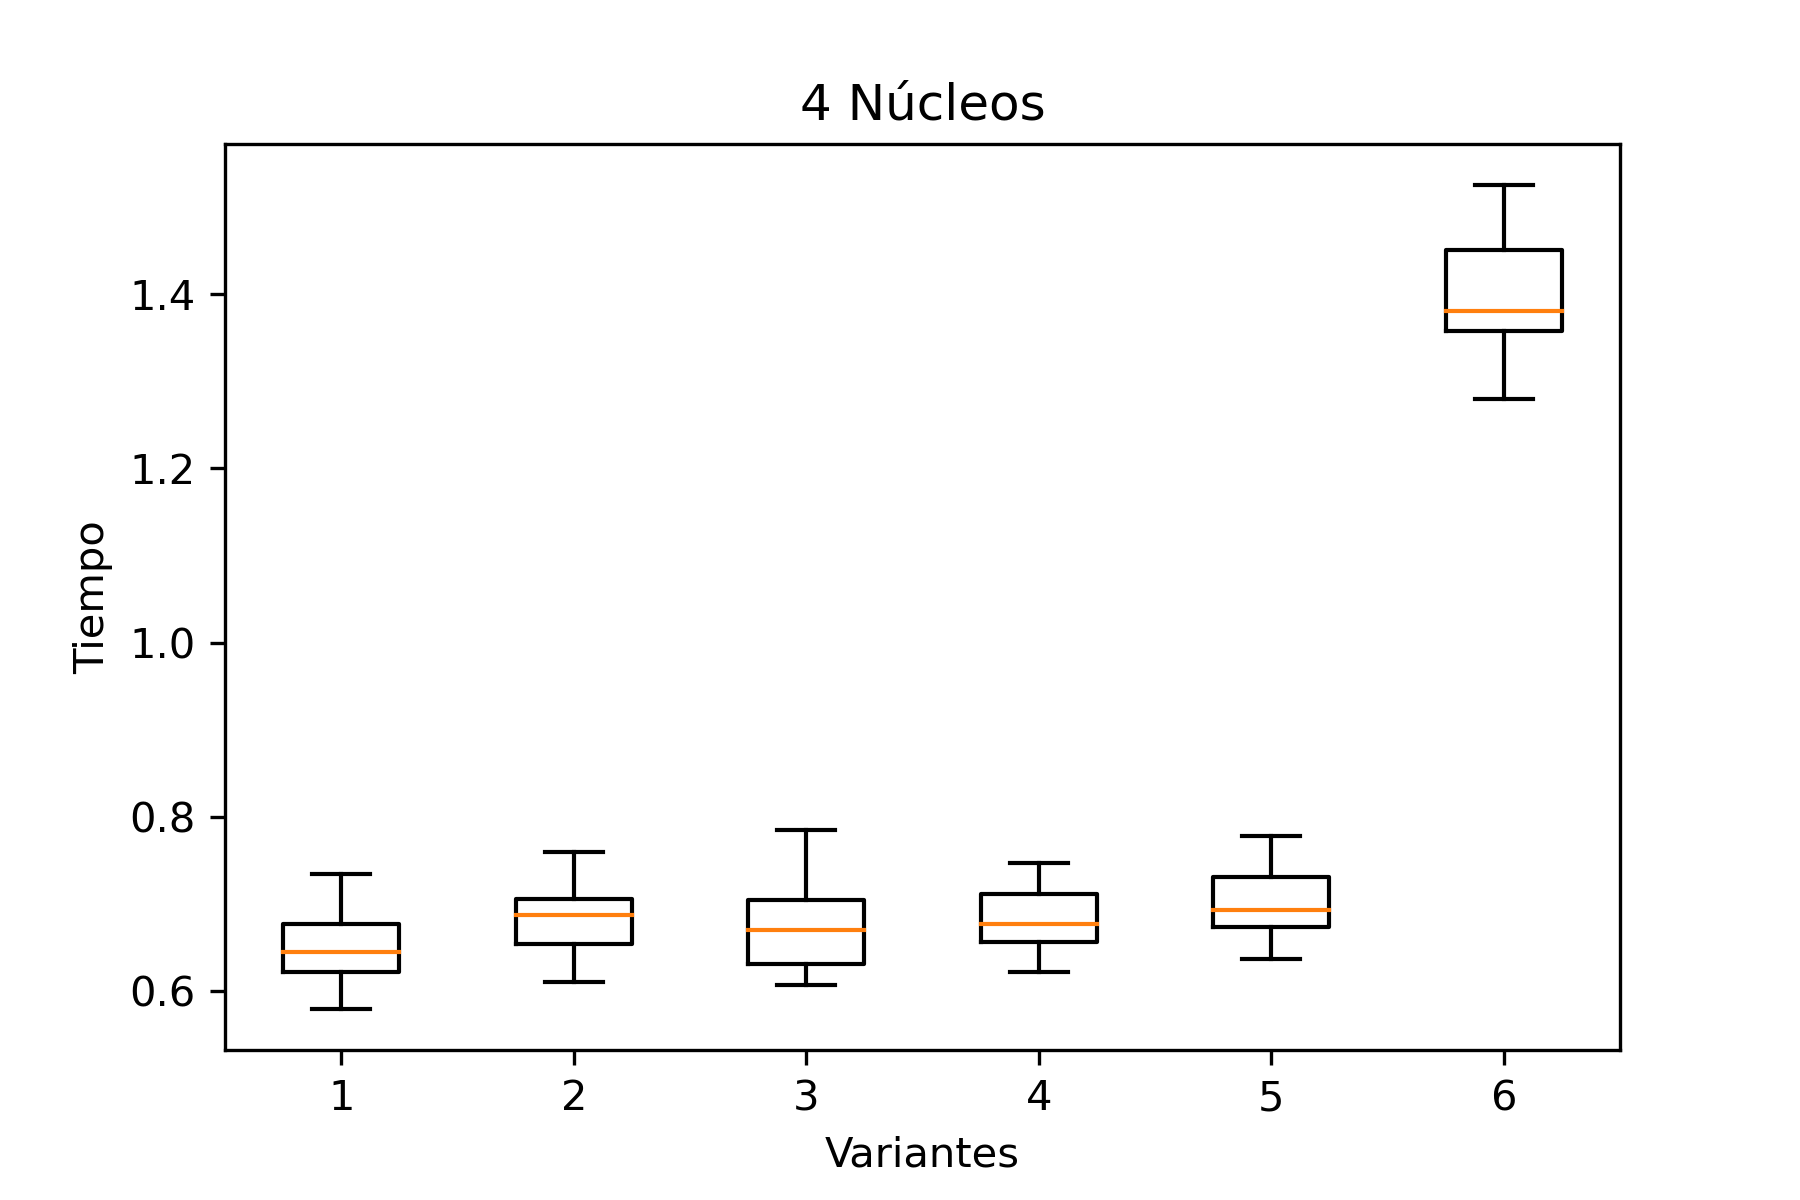
\includegraphics[width=\linewidth]{G_tiempo_4.png}
\caption{Tiempo vs variante con cuatro núcleos}
\end{subfigure}
\caption{Gráfica de tiempo vs variante núcleo 3 y 4 para obtención de números primos y sus potencias.}
\label{fig:westminster}
\end{figure}

\begin{figure}[H]
\centering
\begin{subfigure}[b]{0.45\linewidth}
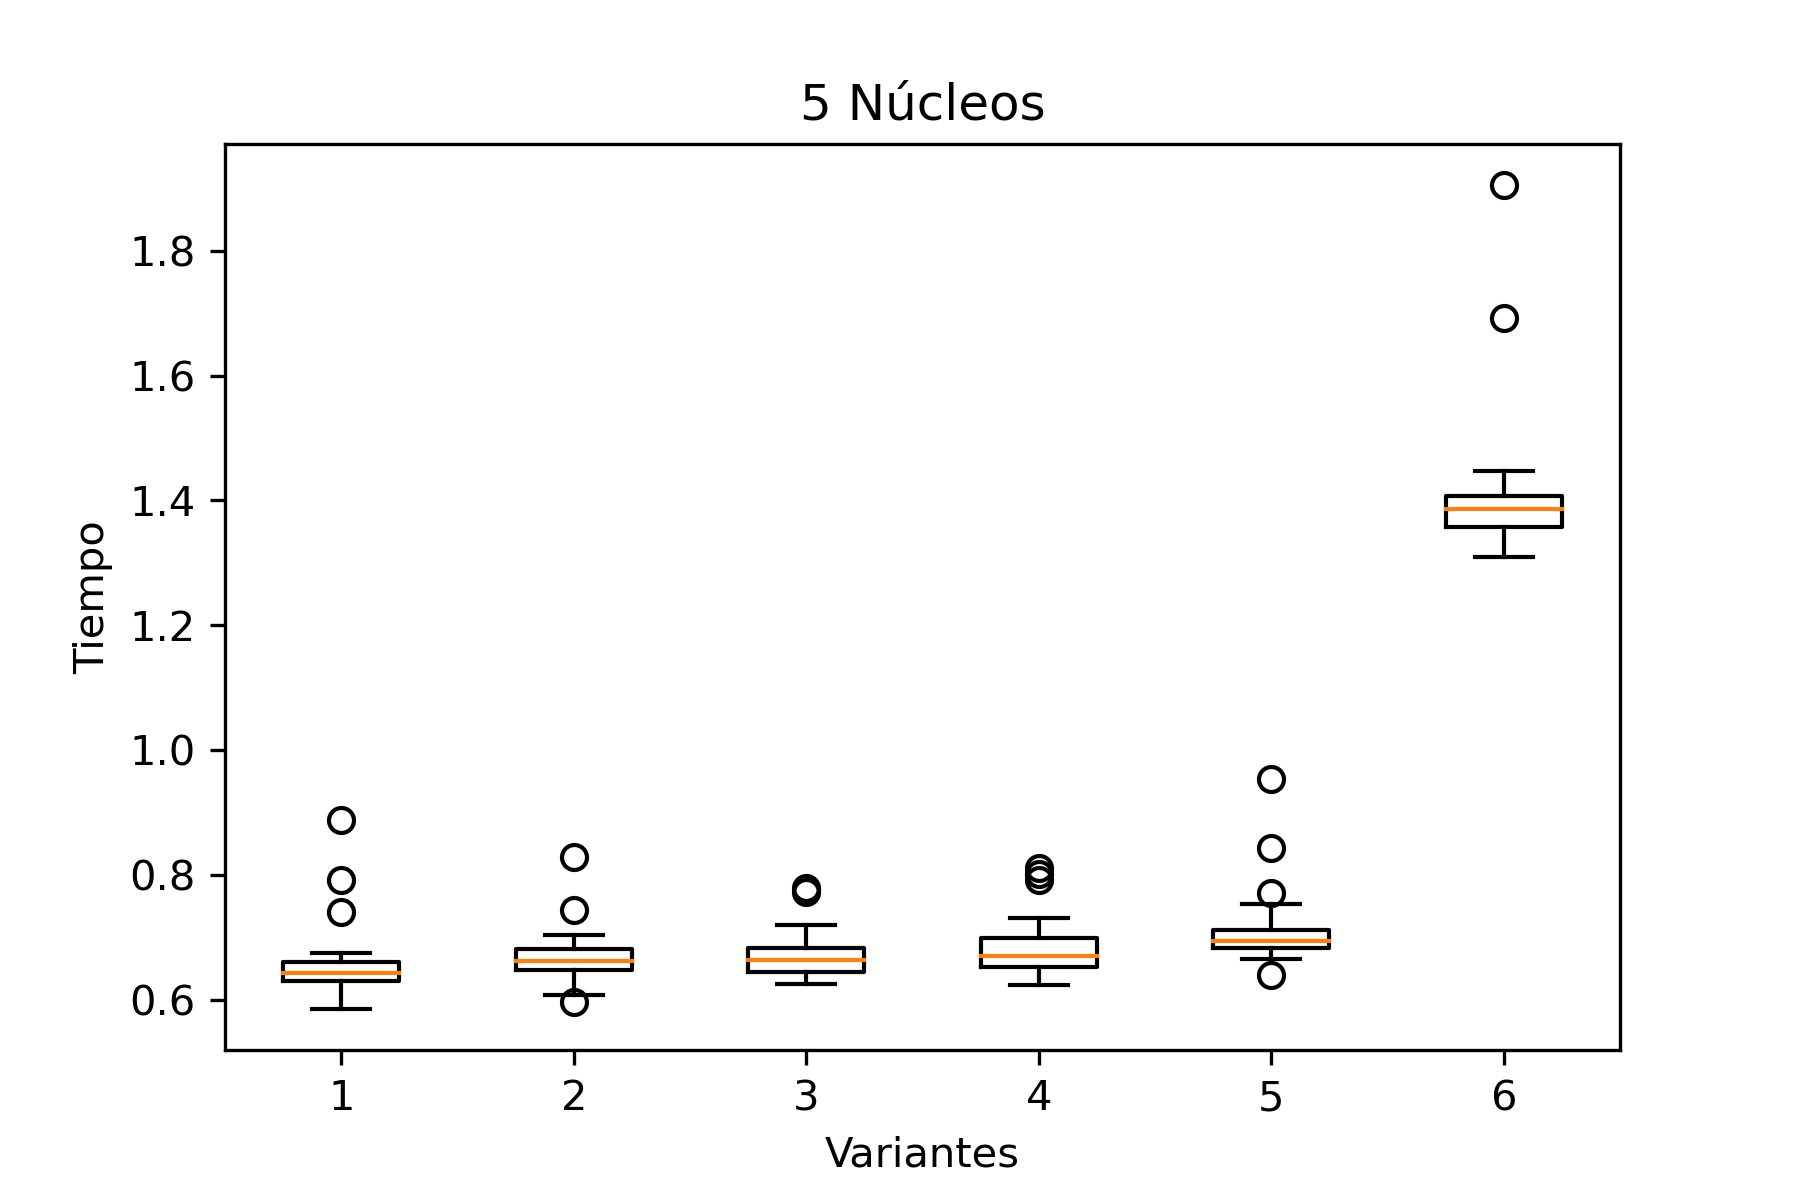
\includegraphics[width=\linewidth]{G_tiempo_5.png}
\caption{Tiempo vs variante con cinco núcleos}
\end{subfigure}
\begin{subfigure}[b]{0.45\linewidth}
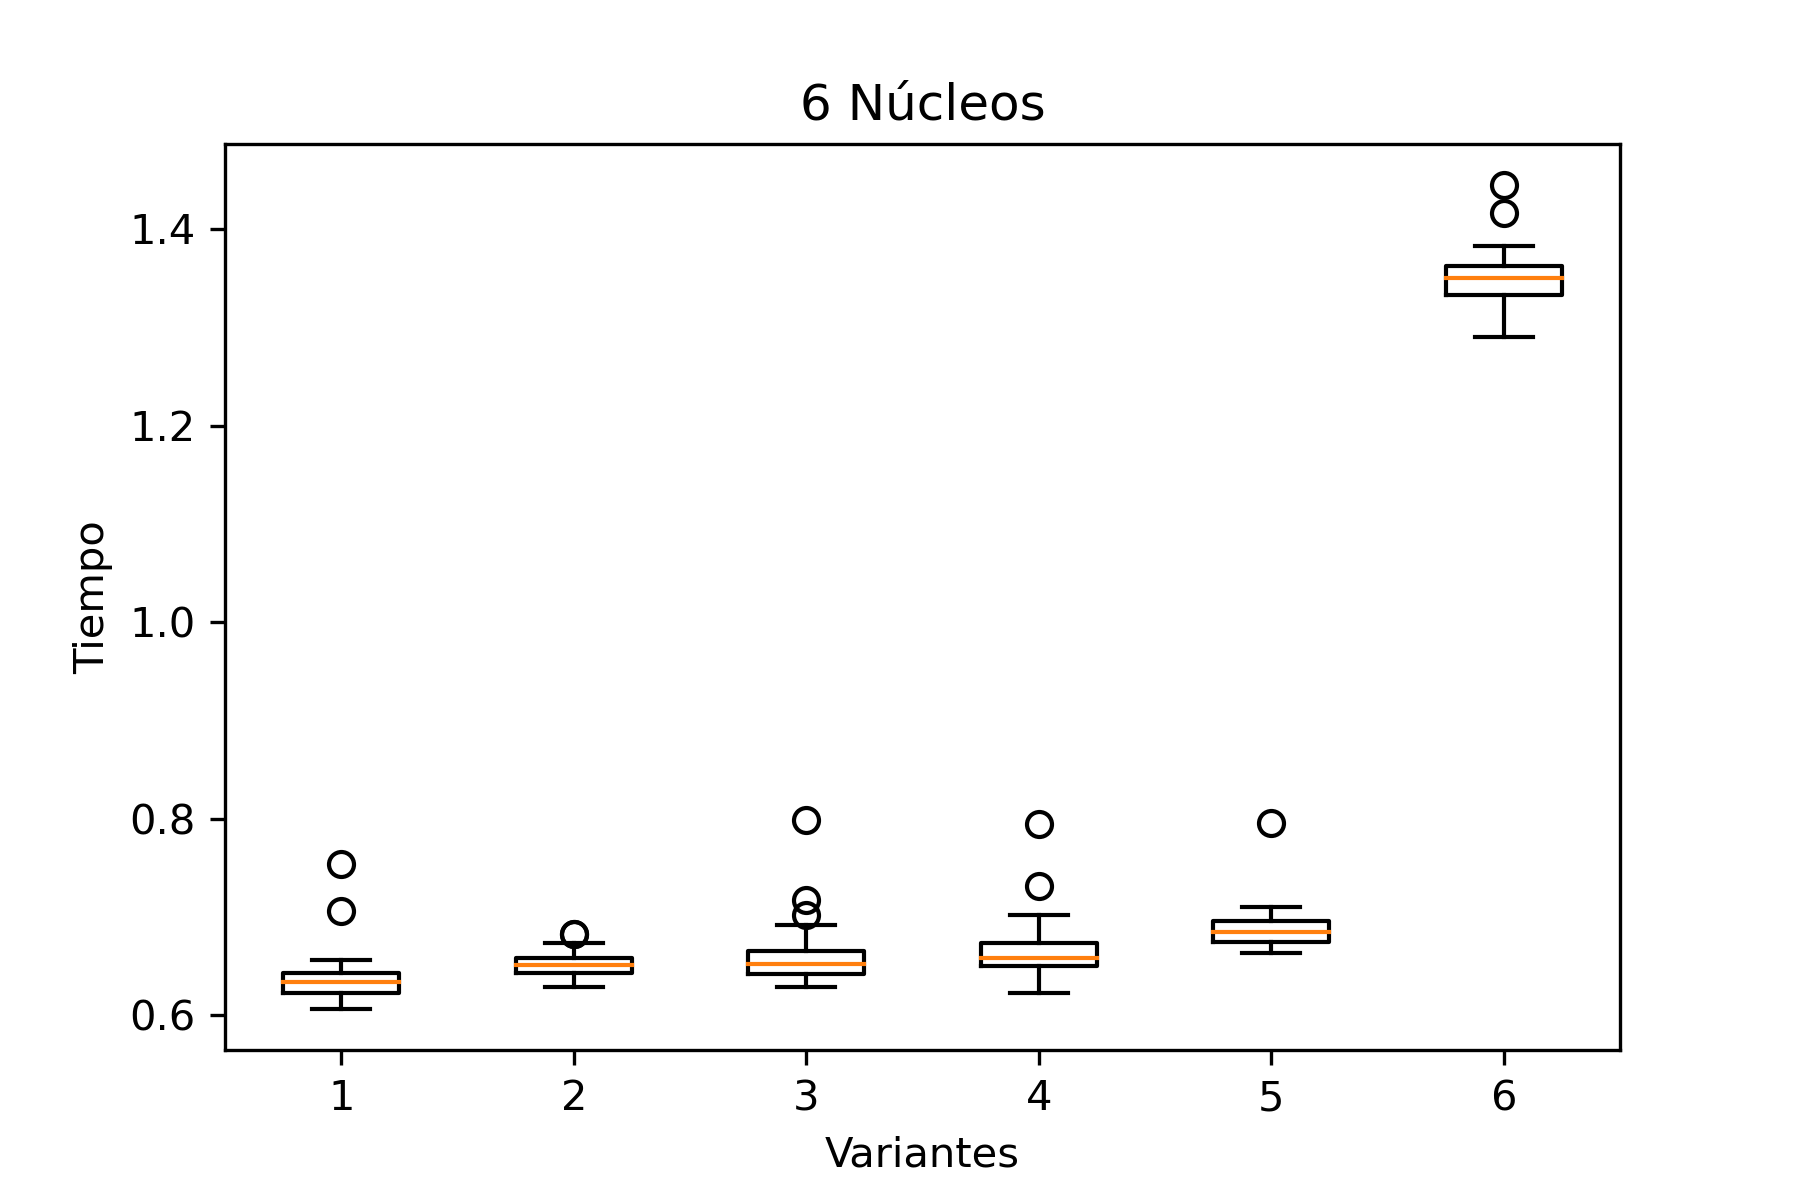
\includegraphics[width=\linewidth]{G_tiempo_6.png}
\caption{Tiempo vs variante con seis núcleos}
\end{subfigure}
\caption{Gráfica de tiempo vs variante núcleo 5 y 6 para obtención de números primos y sus potencias.}
\label{fig:westminster}
\end{figure}

\begin{table}[H]
\begin{center}
\begin{tabular}{|l | r | r | r | r | r | r|}
\hline
\multicolumn{7}{|c|}{Un núcleo}\\
\hline
Variante&iteración&Min-Max&Mediana&Varianza&Asimetría&Curtosis\\
\hline
 Primos               & 40 & 1.50, 1.89  & 1.57 & 0.00 & 2.82   & 9.94\\
 Primos - No primos   & 40 & 1.52, 1.75  & 1.63 & 0.00 & 0.88   & 1.04\\
 No primos - primos   & 40 & 1.57, 1.72  & 1.62 & 0.00 & 0.83   & 0.35\\
 Aleatorio            & 40 & 1.57, 1.95  & 1.64 & 0.00 & 3.05   & 12.68\\
 No primos            & 40 & 1.64, 1.83  & 1.71 & 0.00 & 1.20   & 0.96\\
 Pares                & 40 & 3.25, 3.55  & 3.37 & 0.00 & 0.70   & 0.20\\
\hline
\end{tabular}
\caption{Tabla de estadística con un núcleo}
\label{table:1}
\end{center}
\end{table}

\begin{table}[H]
\begin{center}
\begin{tabular}{|l | r | r | r | r | r | r|}
\hline
\multicolumn{7}{|c|}{Dos núcleos}\\
\hline
Variante&iteración&Min-Max&Mediana&Varianza&Asimetría&Curtosis\\
\hline
 Primos               & 40 & 0.80, 1.00  & 0.86 & 0.00 & 2.10   & 5.57\\
 Primos - No primos   & 40 & 0.86, 1.11  & 0.90 & 0.00 & 2.84   & 8.87\\
 No primos - primos   & 40 & 0.84, 1.09  & 0.90 & 0.00 & 3.14   & 12.78\\
 Aleatorio            & 40 & 0.84, 1.02  & 0.90 & 0.00 & 1.61   & 3.45\\
 No primos            & 40 & 0.86, 1.15  & 0.93 & 0.00 & 3.27   & 15.08\\
 Pares                & 40 & 1.74, 2.34  & 1.86 & 0.01 & 3.15   & 11.90\\
\hline
\end{tabular}
\caption{Tabla de estadística con dos núcleos}
\label{table:1}
\end{center}
\end{table}

\begin{table}[H]
\begin{center}
\begin{tabular}{|l | r | r | r | r | r | r|}
\hline
\multicolumn{7}{|c|}{Tres núcleos}\\
\hline
Variante&iteración&Min-Max&Mediana&Varianza&Asimetría&Curtosis\\
\hline
 Primos               & 40 & 0.67, 0.86  & 0.70 & 0.00 & 2.93   & 9.66\\
 Primos - No primos   & 40 & 0.70, 0.90  & 0.74 & 0.00 & 2.69   & 8.55\\
 No primos - primos   & 40 & 0.70, 0.89  & 0.73 & 0.00 & 3.12   & 11.99\\
 Aleatorio            & 40 & 0.70, 0.81  & 0.74 & 0.00 & 0.99   & 0.33\\
 No primos            & 40 & 0.74, 1.02  & 0.77 & 0.00 & 4.40   & 20.91\\
 Pares                & 40 & 1.46, 1.64  & 1.52 & 0.00 & 1.52   & 1.83\\
\hline
\end{tabular}
\caption{Tabla de estadística con tres núcleos}
\label{table:1}
\end{center}
\end{table}

\begin{table}[H]
\begin{center}
\begin{tabular}{|l | r | r | r | r | r | r|}
\hline
\multicolumn{7}{|c|}{Cuatro núcleos}\\
\hline
Variante&iteración&Min-Max&Mediana&Varianza&Asimetría&Curtosis\\
\hline
 Primos               & 40 & 0.58, 0.73  & 0.64 & 0.00 & 0.18   & -0.28\\
 Primos - No primos   & 40 & 0.61, 0.75  & 0.68 & 0.00 & -0.13   & 0.64\\
 No primos - primos   & 40 & 0.60, 0.78  & 0.67 & 0.00 & 0.38   & -0.38\\
 Aleatorio            & 40 & 0.62, 0.74  & 0.68 & 0.00 & 0.20   & 1.01\\
 No primos            & 40 & 0.63, 0.77  & 0.70 & 0.00 & 0.28   & -0.74\\
 Pares                & 40 & 1.28, 1.52  & 1.39 & 0.00 & 0.27   & -0.72\\
\hline
\end{tabular}
\caption{Tabla de estadística con cuatro núcleos}
\label{table:1}
\end{center}
\end{table}

\begin{table}[H]
\begin{center}
\begin{tabular}{|l | r | r | r | r | r | r|}
\hline
\multicolumn{7}{|c|}{Cinco núcleos}\\
\hline
Variante&iteración&Min-Max&Mediana&Varianza&Asimetría&Curtosis\\
\hline
 Primos               & 40 & 0.58, 0.88  & 0.65 & 0.00 & 2.95   & 10.06\\
 Primos - No primos   & 40 & 0.59, 0.82  & 0.66 & 0.00 & 1.85   & 6.94\\
 No primos - primos   & 40 & 0.62, 0.77  & 0.67 & 0.00 & 1.39   & 2.10\\
 Aleatorio            & 40 & 0.62, 0.81  & 0.68 & 0.00 & 1.40   & 1.84\\
 No primos            & 40 & 0.64, 0.95  & 0.70 & 0.00 & 3.11   & 11.38\\
 Pares                & 40 & 1.30, 1.90  & 1.40 & 0.01 & 3.76   & 15.12\\
\hline
\end{tabular}
\caption{Tabla de estadística con cinco núcleos}
\label{table:1}
\end{center}
\end{table}

\begin{table}[H]
\begin{center}
\begin{tabular}{|l | r | r | r | r | r | r|}
\hline
\multicolumn{7}{|c|}{Seis núcleos}\\
\hline
Variante&iteración&Min-Max&Mediana&Varianza&Asimetría&Curtosis\\
\hline
 Primos               & 40 & 0.60, 0.75  & 0.63 & 0.00 & 2.96   & 10.79\\
 Primos - No primos   & 40 & 0.62, 0.68  & 0.65 & 0.00 & 0.48   & -0.08\\
 No primos - primos   & 40 & 0.62, 0.79  & 0.65 & 0.00 & 2.80   & 10.21\\
 Aleatorio            & 40 & 0.62, 0.79  & 0.66 & 0.00 & 2.44   & 8.24\\
 No primos            & 40 & 0.66, 0.79  & 0.68 & 0.00 & 3.04   & 13.15\\
 Pares                & 40 & 1.28, 1.44  & 1.34 & 0.00 & 1.00   & 2.63\\
\hline
\end{tabular}
\caption{Tabla de estadística con seis núcleos}
\label{table:1}
\end{center}
\end{table}
\printbibliography
\end{document}
